\chapter{Espacios Topológicos}

\section{La topología de $\bb{R}^n$. Los Espacios Métricos}
\begin{definicion}
    Se define el conjunto $\bb{R}^n$ de la siguiente forma:
    \begin{equation*}
        \bb{R}^n = \{x=(x_1,\dots,x_n)\mid x_i\in \bb{R},~i\in \{1,\dots,n\}\}\qquad n\in \bb{N}=\{1,2,3,\dots\}
    \end{equation*}
\end{definicion}

\begin{definicion}[Producto escalar]
    Se define el producto escalar como:
    \Func{\langle,\rangle}{\bb{R}^n\times \bb{R}^n}{\bb{R}}{(x,y)}{\displaystyle \langle x,y\rangle = \langle x,y\rangle = \sum\limits_{i=1}^n x_iy_i}
\end{definicion}

\begin{definicion}[Norma euclídea]
    Se define la norma euclídea o norma usual en $\bb{R}^n$ como:
    \Func{\|\cdot \|_2}{\bb{R}^n}{\bb{R}^+_0}{x}{\displaystyle \|x\|_2 = \sqrt{\langle x,x\rangle} = \sqrt{\sum_{i=1}^n x_i^2}}
\end{definicion}

Asociada a $\|\cdot\|_2$ tenemos la \textbf{distancia} euclídea o usual en $\bb{R}^n$:
\Func{d_2}{\bb{R}^n\times \bb{R}^n}{\bb{R}}{(x,y)}{d_2(x,y)=\|y-x\|_2}

\begin{notacion}
    En el caso de que no se especifique subíndice en la distancia, nos referiremos a la distancia euclídea.
\end{notacion}

Algunas propiedades que se verifican de la distancia son:
\begin{enumerate}
    \item $d(x,y)\geq 0, \quad \forall x,y\in \bb{R}^n$. Además, $d_2(x,y)=0\Longleftrightarrow x=y$.

    \item Simetría: $d_2(x,y)=d_2(y,x),\quad \forall x,y\in \bb{R}^n$.

    \item Desigualdad triangular: $d_2(x,z)\leq d_2(x,y)+d_2(y,z), \quad \quad \forall x,y,z\in \bb{R}^n.$
\end{enumerate}

\begin{ejemplo}
    Para $\bb{R}$ ($n=1$), se tiene que:
    \begin{equation*}
        \|x\|_2 = |x| \hspace{1cm} d(x,y)=|y-x| \qquad \forall x,y\in \bb{R}
    \end{equation*}
\end{ejemplo}

\begin{definicion}[Bola] Sea $x\in \bb{R}^n$ y consideramos $r\in \bb{R}^+$. Se definen:
    \begin{itemize}
        \item \textbf{Bola (abierta)} de centro $x$ y radio $r$ como:
        \begin{equation*}
            B(x,r) = \{y\in \bb{R}^n \mid d(y,x)<r\}
        \end{equation*}

        \item \textbf{Bola cerrada} de centro $x$ y radio $r$ como:
        \begin{equation*}
            \overline{B}(x,r) = \{y\in \bb{R}^n \mid d(y,x)\leq r\}
        \end{equation*}
    \end{itemize}

    En el caso de que simplemente se mencione una bola, sin especificar si es abierta o cerrada, nos referiremos a la bola abierta.
\end{definicion}

\begin{definicion}[Esfera] Sea $x\in \bb{R}^n$ y consideramos $r\in \bb{R}^+$. Se define la esfera de centro $x$ y radio $r$ como:
    \begin{equation*}
        S(x,r) = \{y\in \bb{R}^n \mid d(y,x)=r\}
    \end{equation*}
\end{definicion}

\begin{ejemplo} Algunos ejemplos de bolas y esferas son:
    \begin{enumerate}
        \item Para $\bb{R}$ ($n=1$), consideramos $x\in \bb{R}$ y $r\in \bb{R}^+$. Entonces:
        \begin{gather*}
            B(x,r)=]x-r, x+r[ \\
            \overline{B}(x,r)=[x-r, x+r] \\
            S(x,r)=\{x-r, x+r\}
        \end{gather*}

        \item Para $\bb{R}^2$ ($n=2$), consideramos $x\in \bb{R}^2$ y $r\in \bb{R}^+$. Entonces:
        \begin{figure}[H]
            \begin{subfigure}[b]{0.3\textwidth}
                \centering
                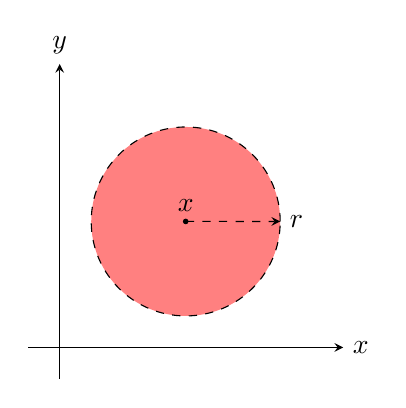
\begin{tikzpicture}[scale=0.8]
                    % Define el centro del círculo en coordenadas (x, y)
                    \coordinate (center) at (2,2);
                    
                    % Define el radio del círculo
                    \def\radius{1.5cm}
                    
                    % Dibuja los ejes
                    \draw[-stealth] (-0.5,0) -- (4.5,0) node[right] {$x$};
                    \draw[-stealth] (0,-0.5) -- (0,4.5) node[above] {$y$};
                    
                    % Dibuja el círculo
                    \draw[dashed, fill=red!50] (center) circle (\radius);
                    \draw[fill=black] (center) circle (1pt); 

                    
                    % Etiqueta el centro
                    \node[above] at (center) {$x$};

                    % Dibuja el radio
                    \draw[dashed, -stealth] (center) --  (3.5,2) node [right]{$r$};
                \end{tikzpicture}
                \caption{$B(x,r)$.\\{\centering Podemos ver que el círculo se incluye pero la circunferencia no.}}
            \end{subfigure}
            \hfill
            \begin{subfigure}[b]{0.3\textwidth}
                \centering
                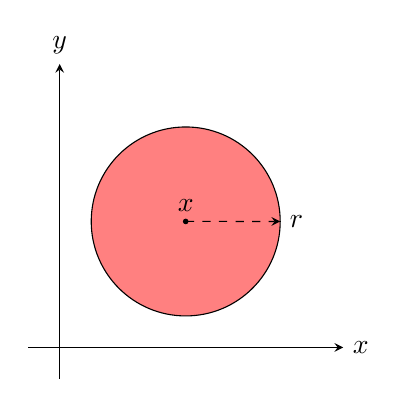
\begin{tikzpicture}[scale=0.8]
                    % Define el centro del círculo en coordenadas (x, y)
                    \coordinate (center) at (2,2);
                    
                    % Define el radio del círculo
                    \def\radius{1.5cm}
                    
                    % Dibuja los ejes
                    \draw[-stealth] (-0.5,0) -- (4.5,0) node[right] {$x$};
                    \draw[-stealth] (0,-0.5) -- (0,4.5) node[above] {$y$};
                    
                    % Dibuja el círculo
                    \draw[fill=red!50] (center) circle (\radius);
                    \draw[fill=black] (center) circle (1pt); 

                    
                    % Etiqueta el centro
                    \node[above] at (center) {$x$};

                    % Dibuja el radio
                    \draw[dashed, -stealth] (center) --  (3.5,2) node [right]{$r$};
                \end{tikzpicture}
                \caption{$\overline{B}(x,r)$. \\{\centering Podemos ver que el círculo se incluye y la circunferencia también.}}
            \end{subfigure}
            \hfill
            \begin{subfigure}[b]{0.3\textwidth}
                \centering
                \begin{tikzpicture}[scale=0.8]
                    % Define el centro del círculo en coordenadas (x, y)
                    \coordinate (center) at (2,2);
                    
                    % Define el radio del círculo
                    \def\radius{1.5cm}
                    
                    % Dibuja los ejes
                    \draw[-stealth] (-0.5,0) -- (4.5,0) node[right] {$x$};
                    \draw[-stealth] (0,-0.5) -- (0,4.5) node[above] {$y$};
                    
                    % Dibuja el círculo
                    \draw (center) circle (\radius);
                    
                    % Etiqueta el centro
                    \draw[fill=black] (center) circle (1pt); 
                    \node[above] at (center) {$x$};

                    % Dibuja el radio
                    \draw[dashed, -stealth] (center) --  (3.5,2) node [right]{$r$};
                \end{tikzpicture}
                \caption{$S(x,r)$. \\{\centering Podemos ver que solo se incluye el círculo. La circunferencia no se incluye.}}
            \end{subfigure}
            \caption{Bolas y esferas en el caso de $\bb{R}^2$ ($n=2$).}
        \end{figure}
        
        \begin{samepage}
        \item Para $\bb{R}^3$ ($n=3$), consideramos $x\in \bb{R}^3$ y $r\in \bb{R}^+$. Entonces:
        \begin{figure}[H]
            \begin{subfigure}[b]{0.3\textwidth}
                \centering
                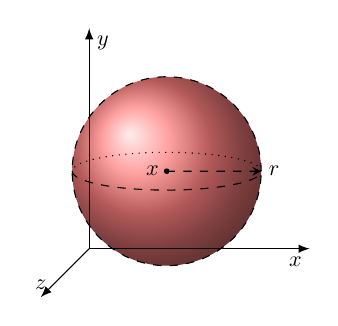
\begin{tikzpicture}[scale=0.8,transform shape]            
                    \def\r{1.5}
                    \def\b{0.3}
        
                    \coordinate (center) at (2,2,2);
                
                    % Dibuja la esfera con el interior rojo
                    \shade[ball color=red!50] (center) circle (\r);
                
                    % Dibuja el borde en negro
                    \draw[dashed] (center) circle (\r);
                
                    \draw[dashed] (-\r+2,2,2) arc (180:360:\r cm and \b cm);
                    \draw[dotted] (\r+2,2,2) arc (0:180:\r cm and \b cm);
        
                    % Etiqueta el centro
                    \draw[fill=black] (center) circle (1pt); 
                    \node[left] at (center) {$x$};
        
                    % Dibuja el radio
                    \draw[dashed, -stealth] (center) --  (2+\r,2,2) node [right]{$r$};
        
                    
                    % Ejes 3D
                    \draw[-latex] (0,0,0) -- (3.5,0,0) node[anchor=north east]{$x$};
                    \draw[-latex] (0,0,0) -- (0,3.5,0) node[anchor=north west]{$y$};
                    \draw[-latex] (0,0,0) -- (0,0,2) node[anchor=south]{$z$};
                \end{tikzpicture}
                \caption{$B(x,r)$.\\{\centering Podemos ver que el interior se incluye pero el borde no.}}
            \end{subfigure}
            \hfill
            \begin{subfigure}[b]{0.3\textwidth}
                \centering
                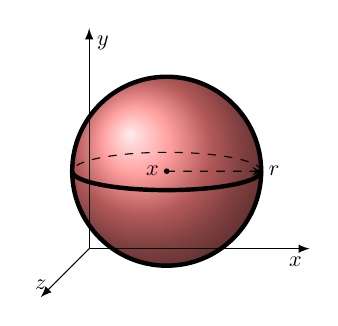
\begin{tikzpicture}[scale=0.8,transform shape]            
                    \def\r{1.5}
                    \def\b{0.3}
        
                    \coordinate (center) at (2,2,2);
                
                    % Dibuja la esfera con el interior rojo
                    \shade[ball color=red!50] (center) circle (\r);
                
                    % Dibuja el borde en negro
                    \draw[ultra thick] (center) circle (\r);
                
                    \draw[ultra thick] (-\r+2,2,2) arc (180:360:\r cm and \b cm);
                    \draw[dashed] (\r+2,2,2) arc (0:180:\r cm and \b cm);
        
                    % Etiqueta el centro
                    \draw[fill=black] (center) circle (1pt); 
                    \node[left] at (center) {$x$};
        
                    % Dibuja el radio
                    \draw[dashed, -stealth] (center) --  (2+\r,2,2) node [right]{$r$};
        
                    
                    % Ejes 3D
                    \draw[-latex] (0,0,0) -- (3.5,0,0) node[anchor=north east]{$x$};
                    \draw[-latex] (0,0,0) -- (0,3.5,0) node[anchor=north west]{$y$};
                    \draw[-latex] (0,0,0) -- (0,0,2) node[anchor=south]{$z$};
                \end{tikzpicture}
                \caption{$\overline{B}(x,r)$. \\{\centering Podemos ver que el interior y el borde se incluyen.}}
            \end{subfigure}
            \hfill
            \begin{subfigure}[b]{0.3\textwidth}
                \centering
                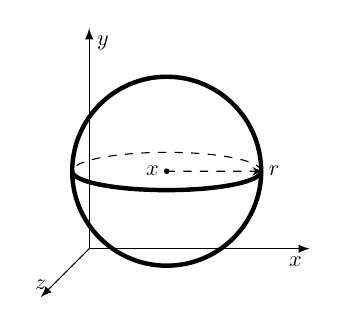
\begin{tikzpicture}[scale=0.8,transform shape]            
                    \def\r{1.5}
                    \def\b{0.3}
        
                    \coordinate (center) at (2,2,2);
                
                    % Dibuja el borde en negro
                    \draw[ultra thick] (center) circle (\r);
                
                    \draw[ultra thick] (-\r+2,2,2) arc (180:360:\r cm and \b cm);
                    \draw[dashed] (\r+2,2,2) arc (0:180:\r cm and \b cm);
        
                    % Etiqueta el centro
                    \draw[fill=black] (center) circle (1pt); 
                    \node[left] at (center) {$x$};
        
                    % Dibuja el radio
                    \draw[dashed, -stealth] (center) --  (2+\r,2,2) node [right]{$r$};
        
                    
                    % Ejes 3D
                    \draw[-latex] (0,0,0) -- (3.5,0,0) node[anchor=north east]{$x$};
                    \draw[-latex] (0,0,0) -- (0,3.5,0) node[anchor=north west]{$y$};
                    \draw[-latex] (0,0,0) -- (0,0,2) node[anchor=south]{$z$};
                \end{tikzpicture}
                \caption{$S(x,r)$. \\{\centering Podemos ver que solo se incluye el borde.}}
            \end{subfigure}
            \caption{Bolas y esferas en el caso de $\bb{R}^3$ ($n=3$).}
        \end{figure}
        \end{samepage}
    \end{enumerate}
\end{ejemplo}


De las definiciones, se deduce de forma directa y trivial la siguiente proposición:
\begin{prop}
    Sea $x\in \bb{R}^n$ y consideramos $r\in \bb{R}^+$. Tenemos que:
    \begin{enumerate}
        \item $\ol{B}(x,r)=B(x,r)\cup S(x,r)$,
        \item $S(x,r)=\ol{B}(x,r)\setminus S(x,r)$,
        \item Sea $s\in \bb{R}$. Si $r<s$, entonces $\ol{B}(x,r)\subset B(x,s)$.
    \end{enumerate}
\end{prop}

A continuación, veamos que las bolas son de gran utilidad para la convergencia de sucesiones. Recordemos la definición de sucesión convergente:
\begin{definicion}
    Una sucesión $\{x_n\}$ es convergente a un límite $x_0$ si:
    \begin{equation*}
        \forall \veps\in \bb{R}^+,\quad \exists j_0\in \bb{N}\mid |x_j-x_0|<\veps \quad \forall j>j_0 
    \end{equation*}
\end{definicion}

\begin{observacion}
    Notemos que, usando el concepto de distancia, una sucesión $\{x_n\}$ es convergente a un límite $x_0$ si:
    \begin{equation*}
        \forall \veps\in \bb{R}^+,\quad \exists j_0\in \bb{N}\mid d(x_j,x_0)<\veps \quad \forall j>j_0 
    \end{equation*}

    Notemos que, usando el concepto de bola, una sucesión $\{x_n\}$ es convergente a un límite $x_0$ si:
        \begin{equation*}
            \forall \veps\in \bb{R}^+,\quad \exists j_0\in \bb{N}\mid x_j\in B(x_0,\veps) \quad \forall j>j_0 
        \end{equation*}
\end{observacion}


Veamos ahora lo análogo para el caso de la continuidad de funciones:
\begin{definicion}
    Una sucesión $f:I\subset \bb{R}\to \bb{R}$ es continua en $x_0\in I$ si:
    \begin{equation*}
        \forall \veps\in \bb{R}^+,\quad \exists \delta>0 \mid |f(x)-f(x_0)|<\veps \quad \forall x\in I,~|x-x_0|< \delta 
    \end{equation*}
\end{definicion}

\begin{observacion}
    Notemos que, usando el concepto de distancia, dado $I\subset \bb{R}$, la función $f:I\to \bb{R}$ es continua en $x_0\in I$ si:
    \begin{equation*}
        \forall \veps\in \bb{R}^+,\quad \exists \delta>0 \mid d[f(x)-f(x_0)]<\veps \quad \forall x\in I,~d[f(x)-f(x_0)]< \delta 
    \end{equation*}

    Notemos que, usando el concepto de bola, una función $f:I\subset \bb{R}\to \bb{R}$ es continua en $x_0\in I$ si:
        \begin{equation*}
            \forall \veps\in \bb{R}^+,\quad \exists \delta>0 \mid f[B(x_0,\delta)]\subset B[f(x_0,\veps)]
        \end{equation*}
\end{observacion}


\begin{definicion} [Espacio Métrico]
    Sea $X\neq \emptyset$ un cojunto no vacío. Un espacio métrico es un par $(X,d)$ donde $d:X\times X\to \bb{R}$ cumple:
    \begin{description}
        \item[D1)] $d(x,y)\geq 0, \quad \forall x,y\in X$. Además, se tiene que $d(x,y)=0\Longleftrightarrow x=y$.

        \item[D2)] $d(x,y)=d(y,x), \quad \forall x,y\in X$.

        \item[D3)] $d(x,z)\leq d(x,y)+d(y,z),\quad \forall x,y,z\in X$.
    \end{description}

    A la aplicación $d$ se le denomina \textbf{distancia} en $X$.
\end{definicion}

\begin{observacion}
    Los apartados D2, D3 y la segunda parte de D1 implican la primera parte de D1. Para verlo, sean $x,y\in X$:
    \begin{equation*}
        0\stackrel{2^a~D1}{=} d(x,x) \stackrel{D3}\leq d(x,y) + d(y,x) \stackrel{D2}{=} 2d(x,x)
    \end{equation*}
\end{observacion}

En un espacio métrico también se definen las bolas y las esferas definidas en el caso de los reales. Sea $(X,d)$ un espacio métrico. Sea $x\in X$ y consideramos $r\in \bb{R}^+$. Entonces:
\begin{itemize}
    \item $B(x,r) = \{y\in X \mid d(y,x)<r\}$
    \item $\overline{B}(x,r) = \{y\in X \mid d(y,x)\leq r\}$
    \item $S(x,r) = \{y\in X \mid d(y,x)=r\}$
\end{itemize}

\begin{notacion}
    Notamos $\bb{S}^n=S(x,1)\subset \bb{R}^{n+1}$, donde $x=(0,\dots,0)\in \bb{R}^{n+1}$.
\end{notacion}


\begin{definicion}[Espacio Normado]
    Sea $V$ un espacio vectorial real. Un espacio normado es un par $(V,\|\cdot\|)$ donde $\|\cdot\|:V\to \bb{R}$ cumple:
    \begin{description}
        \item[N1)] $\|v\|\geq 0, \quad \forall v\in V$. Además, se tiene que $\|v\|=0\Longleftrightarrow v=0$.

        \item[N2)] $\|\lambda v\| = |\lambda|\|v\|, \quad \forall v\in V, \lambda\in \bb{R}$.

        \item[N3)] $\|u+v\|\leq \|u\|+\|v\|,\quad \forall u,v\in V$. Se denomina desigualdad de Minkowski.
    \end{description}
    Diremos que $\|\cdot\|$ es una \textbf{norma en $V$}.
\end{definicion}

\begin{observacion}
    Los apartados N2, N3 y la segunda parte de N1 implican la primera parte de N1. Para verlo, sea $v\in V$:
    \begin{equation*}
        0\stackrel{2^a~N1}{=} \|v+(-v)\| \stackrel{N3}\leq \|v\|+\|-v\| \stackrel{N2}{=} 2\|v\|
    \end{equation*}
\end{observacion}

\begin{prop}
    Todo espacio normado $(V,\|\cdot\|)$ es también un espacio métrico con $$d(u,v)=\|v-u\|,\quad \forall u,v\in V$$
    A $d$ se le denomina distancia asociada a (o inducida por) la norma, y se denota por $d_{\|~\|}$.
\end{prop}
\begin{proof}
    Veamos que la distancia así definida es una distancia:
    \begin{enumerate}
        \item $d(u,v)=||v-u||\geq 0$. Además, se tiene que $$d(u,v)=||v-u||=0\Longleftrightarrow v-u=0 \Longleftrightarrow v=u$$
        \item $d(u,v)=||v-u||=|-1|\cdot \|u-v\| = \|u-v\| = d(v,u)$.
        \item $d(u,t)=||t-u|| = ||t-u+v-v|| = ||v-u +t-v||$. Aplicando la desigualdad triangular, tenemos que $d(u,t)\leq ||v-u|| + ||t-v|| = d(u,v) + d(v,t)$.
    \end{enumerate}
    Por tanto, vemos que efectivamente es una distancia y, por tanto, se trata de un espacio métrico.
\end{proof}

\begin{definicion}[Métrica euclídea]
    Una aplicación de denomina por métrica euclídea si es una forma bilineal simétrica y definida positiva.
\end{definicion}

\begin{definicion}[Espacio vectorial euclídeo] Un espacio vectorial euclídeo es un par $(V,~\langle,\rangle)$ donde $V$ es un espacio vectorial real y $\langle,\rangle:V\times V\to \bb{R}$ es una métrica euclídea en $V$.

En él, tenemos la norma y distancia asociada (o inducida):
$$\|v\|=\sqrt{\langle r,r\rangle}\hspace{1cm}d(u,v)=\|v-u\| \hspace{1cm} \forall u,v\in V$$
\end{definicion}

\begin{observacion}
    Se cumple que:
    \begin{equation*}
        \text{E.V. Euclídeos} \subsetneq
        \text{E. normados} \subsetneq
        \text{E. métricos}
    \end{equation*}
\end{observacion}

\begin{ejemplo} Ejemplos de espacios normados son:
\begin{enumerate}
    \item $(\bb{R}^n,~\langle,\rangle)$, con $\langle,\rangle=\sum\limits_{i=1}^n x_iy_i$
    es un espacio vectorial euclídeo con la norma $\|\cdot \|_2.$

    \item En $\bb{R}^n$, para cada $p\in \bb{N}$ se define la norma $p$ como:
    \Func{\|\cdot\|_p}{\bb{R}^n}{\bb{R}}{x}{\sqrt[p]{\sum\limits_{i=1}^n |x_i|^p}}

    Se tiene que $(\bb{R}^n, \|\cdot\|_p)$ es un espacio normado.
    \begin{itemize}
        \item Para $p=2$, se tiene que $\|\cdot\|_2$ es la norma usual.
        \item Para $p=1$, la norma $\|\cdot\|_1$ es la distancia del taxi o métrica de Manhattan.
    \end{itemize}

    \item En $\bb{R}^n$, se define la norma infinito como $\|x\|_\infty = \max\limits_{1\leq i\leq n}\{|x_i|\}$.

    Se tiene que $(\bb{R}^n, \|\cdot\|_\infty)$ es un espacio normado.
\end{enumerate}
\end{ejemplo}

Veamos cómo son las bolas abiertas para las distintas normas presentadas en el anterior ejemplo. Dado $x=(x_1,x_2)\in \bb{R}^2, r\in \bb{R}^+$, se tiene que:
\begin{align*}
    & B_2(x,r)=\{y=(y_1, y_2)\in \bb{R}^2 \mid \sqrt{(x_1-y_1)^2+(x_2-y_2)^2} < r\} \\
    & B_1(x,r)=\{y=(y_1, y_2)\in \bb{R}^2 \mid |x_1-y_1|+|x_2-y_2| < r\} \\
    & B_\infty(x,r)=\{y=(y_1, y_2)\in \bb{R}^2 \mid \max\{|x_1-y_1|,|x_2-y_2|\} < r\}
\end{align*}
\begin{figure}[H]
    \begin{subfigure}[b]{0.3\textwidth}
        \centering
        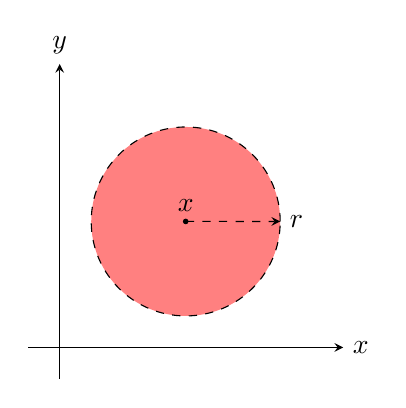
\begin{tikzpicture}[scale=0.8]
            % Define el centro del círculo en coordenadas (x, y)
            \coordinate (center) at (2,2);
            
            % Define el radio del círculo
            \def\radius{1.5cm}
            
            % Dibuja los ejes
            \draw[-stealth] (-0.5,0) -- (4.5,0) node[right] {$x$};
            \draw[-stealth] (0,-0.5) -- (0,4.5) node[above] {$y$};
            
            % Dibuja el círculo
            \draw[dashed, fill=red!50] (center) circle (\radius);
            \draw[fill=black] (center) circle (1pt); 

            
            % Etiqueta el centro
            \node[above] at (center) {$x$};

            % Dibuja el radio
            \draw[dashed, -stealth] (center) --  (3.5,2) node [right]{$r$};
        \end{tikzpicture}
        \caption{$B_2(x,r)$}
    \end{subfigure}
    \hfill
    \begin{subfigure}[b]{0.3\textwidth}
        \centering
        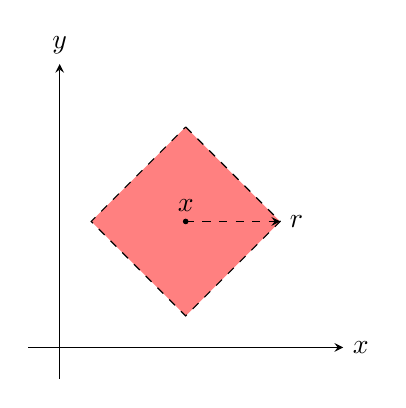
\begin{tikzpicture}[scale=0.8]
            % Define el centro del cuadrado en coordenadas (x, y)
            \def\x{2}
            \def\y{2}
            
            \def\r{1.5}
            
            % Dibuja los ejes
            \draw[-stealth] (-0.5,0) -- (4.5,0) node[right] {$x$};
            \draw[-stealth] (0,-0.5) -- (0,4.5) node[above] {$y$};
            
            % Dibuja el cuadrado
            \draw[dashed, fill=red!50] (\x, \y+\r) -- (\x+\r, \y) -- (\x, \y-\r) -- (\x-\r, \y) -- cycle;
            \draw[fill=black] (\x,\y) circle (1pt); 

            
            % Etiqueta el centro
            \node[above] at (\x,\y) {$x$};

            % Dibuja el radio
            \draw[dashed, -stealth] (\x, \y) --  (\x+\r, \y) node [right]{$r$};
        \end{tikzpicture}
        \caption{${B}_1(x,r)$}
    \end{subfigure}
    \hfill
    \begin{subfigure}[b]{0.3\textwidth}
        \centering
        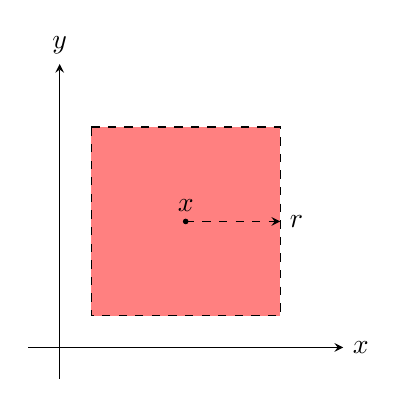
\begin{tikzpicture}[scale=0.8]
            % Define el centro del cuadrado en coordenadas (x, y)
            \def\x{2}
            \def\y{2}
            
            \def\r{1.5}
            
            % Dibuja los ejes
            \draw[-stealth] (-0.5,0) -- (4.5,0) node[right] {$x$};
            \draw[-stealth] (0,-0.5) -- (0,4.5) node[above] {$y$};
            
            % Dibuja el cuadrado
            \draw[dashed, fill=red!50] (\x-\r, \y+\r) -- (\x+\r, \y+\r) -- (\x+\r, \y-\r) -- (\x-\r, \y-\r) -- cycle;
            \draw[fill=black] (\x,\y) circle (1pt); 

            
            % Etiqueta el centro
            \node[above] at (\x,\y) {$x$};

            % Dibuja el radio
            \draw[dashed, -stealth] (\x, \y) --  (\x+\r, \y) node [right]{$r$};
        \end{tikzpicture}
        \caption{${B}_\infty(x,r)$}
    \end{subfigure}
    \caption{Bolas abiertas en el caso de $\bb{R}^2$ ($n=2$) para distintas normas.}
\end{figure}

\begin{ejemplo}
    En el espacio vectorial $V=C^0([a,b], \bb{R})$ de las funciones reales continuas definidas en el intervalo $[a,b]$, con $a<b$ tenemos la métrica euclídea
    \begin{equation*}
        \langle f,g\rangle = \int_a^b f(x)g(x)~dx
    \end{equation*}
    Tenemos que dicho espacio vectorial con esa norma definida es un espacio vectorial euclídeo.
    
    Cabe destacar que dicho espacio vectorial tiene dimensión infinita.
\end{ejemplo}

\begin{ejemplo}
    Sea $X\neq \emptyset$. Se define la distancia discreta en $X$ como $d_{disc}:X\times X\to \bb{R}$ como:
    \begin{equation*}
        d(x,y)=\left\{
            \begin{array}{ccc}
                0 & \text{si} & x=y \\
                1 & \text{si} & x\neq y
            \end{array}
        \right.
    \end{equation*}

    Dado $x\in X, r\in \bb{R}^+$, las bolas y esfera son:
    \begin{equation*}
        B(x,r)=\left\{
            \begin{array}{ccc}
                \{x\} & \text{si} & r \leq 1 \\
                X & \text{si} & r > 1
            \end{array}
        \right.
        \hspace{0.5cm}
        \ol{B}(x,r)=\left\{
            \begin{array}{ccc}
                \{x\} & \text{si} & r < 1 \\
                X & \text{si} & r \geq 1
            \end{array}
        \right.
        \hspace{0.5cm}
        S(x,r)=\left\{
            \begin{array}{ccc}
                X\setminus \{x\} & \text{si} & r = 1 \\
                \emptyset & \text{si} & r \neq 1
            \end{array}
        \right.
    \end{equation*}
\end{ejemplo}

\begin{prop}
    Si $d$ es una distancia en $X$ y $\lambda\in \bb{R}^+$, entonces $\lambda d$ es también una distancia en $X$. Además, se tiene que:
    \begin{equation*}
        B_{\lambda d}(x,r) = B_d\left(x, \frac{r}{\lambda}\right)
    \end{equation*}
\end{prop}
\begin{proof}
    Comprobamos en primer lugar que se trata de una distancia. Para ello ha de cumplir las tres condiciones dadas en la definición de espacio métrico:
    \begin{enumerate}
        \item $\lm d(x,y)\geq 0, \quad \forall x,y\in X$, ya que $\lm>0, d(x,y)\geq 0$. Además, como $\lambda\neq 0$, se tiene que $\lambda d(x,y)=0 \Longleftarrow x=y$.

        \item Trivialmente, se tiene que $\lambda d(x,y)=\lambda d(y,x), \quad \forall x,y\in X$.

        \item $\lambda d(x,z)\leq \lambda d(x,y) + \lambda d(y,z), \quad \forall x,y,z\in X$, ya que al ser $\lm>0$ se puede sacar como factor común y pasar dividiendo sin que afecte al sentido de la desigualdad.
    \end{enumerate}

    Por tanto, tenemos que se trata de una distancia. Comprobemos lo referido a las bolas:
    \begin{equation*}
        B_{\lm d}(x,r)
        = \{y\in X \mid \lambda d(x,y)<r\}
        = \left\{y\in X \mid d(x,y)<\dfrac{r}{\lm}\right\}
        = B_d\left(x, \frac{r}{\lambda}\right)
    \end{equation*}
\end{proof}

\begin{definicion}[Conjunto abierto métrico]
Sea $(X,d)$ espacio métrico. Diremos que un conjunto $U\subset X$ es abierto métrico si $U=\emptyset$, o bien
$$\forall x\in U,~\exists r\in \bb{R}^+\mid B(x,r)\subset U$$

Denotamos $\cc{T}_d=\{U\subset X\mid U\text{ es un abierto métrico en } (X,d)\}\subset \cc{P}(X)$. 
\end{definicion}

\begin{ejemplo}
    En $(\bb{R}^2, d)$, hemos de notar que todo abierta no puede incluir al borde, ya que si se incluyese entonces al escocer un punto del borde no se cumpliría la condición pedida.
\end{ejemplo}


Algunas propiedades de los abiertos son:
\begin{prop} Sea $(X,d)$ un espacio métrico. Entonces:
    \begin{enumerate}
        \item[(A1)] $\emptyset, X\in \cc{T}_d$.
        \item[(A2)] Si $\{U_i\}_{i\in I}\subset \cc{T}_d$, entonces $ \bigcup\limits_{i\in I} U_i\in \cc{T}_d$.
        \item[(A3)] Si $U_1,U_2\in \T_d$, entonces $U_1\cap U_2\in \T_d$.
    \end{enumerate}
\end{prop}
\begin{proof}\
\begin{enumerate}
        \item[(A1)] $\emptyset\in \cc{T}_d$ trivialmente. Además, $X\in \T_d$ debido a que, para todo punto de $X$, se tiene que la bola centrada en él, independientemente del radio, está contenida en el total $X$.
        
        \item[(A2)] Si $\{U_i\}_{i\in I}\subset \cc{T}_d$, entonces $ \bigcup\limits_{i\in I}U_i \in \cc{T}_d$.

        Sea $x\in U=\bigcup\limits_{i\in I}U_i$, por lo que $\exists i\in I\mid x\in U_i$. Por tanto, $\exists r\in \bb{R}^+ $ tal que $ B(x,r)\in U_i\subset U$, por lo que se tiene.
        
        \item[(A3)] Si $U_1,U_2\in \T_d$, entonces $U_1\cap U_2\in \T_d$.

        Sea $x\in U_1\cap U_2$. Entonces, como $x\in U_i$, se tiene que $\exists B(x, r_i)\subset U_i$ con $r_i\in \bb{R}^+$ para $i=1,2$. Supongamos (sin perder generalidad) que $r_1\leq r_2$. Entonces, tenemos que $B(x,r_1)\subseteq B(x,r_2)\subset U_2$. Por tanto, como $B(x,r_1)\subset U_1,U_2$ tenemos que $B(x,r_1)\subset U_1\cap U_2$, por lo que $U_1\cap U_2\in \T_d$.
    \end{enumerate}
\end{proof}

Por la tercera propiedad, la demostración mediante inducción sobre $k$ del siguiente apartado es inmediata:
\begin{coro}
    Sea $(X,d)$ un espacio métrico.
    
    Entonces, si $U_1,\dots, U_k \in \cc{T}_d$, $k\in \bb{N}$ entonces $U_1\cap \dots \cap U_k\in \cc{T}_d$.
\end{coro}

\begin{prop} Sea $(X,d)$ un espacio métrico. Se cumple que todas las bolas abiertas son abiertos métricos.
\end{prop}
\begin{proof}
    Sea la bola abierta $B(x,r)$. Consideramos $y\in B(x,r)$. Veamos si $\exists \veps \in \bb{R}^+\mid B(y,\veps)\subset B(x,r)$.

    Como $d(x,y)<r$ por la elección de $y$, tenemos que $\exists \veps \in \bb{R}^+\mid d(x,y)+\veps<r$. Veamos que $B(y,\veps)\subset B(x,r)$. Considerando $z\in B(y,\veps)$, se tiene que:
    \begin{equation*}
        d(z,x)\leq d(z,y)+d(y,x)\leq \varepsilon + d(x,y)< r
    \end{equation*}

    Por tanto, tenemos que $\exists \veps \in \bb{R}^+\mid B(y,\veps)\subset B(x,r)$, por lo que la bola $B(x,r)$ es un abierto.
\end{proof}

No obstante, el otro sentido de la afirmación no se tiene; es decir, no todo abierto métrico es una bola. Ejemplo de esto es $\bb{R}^n$.

\begin{observacion}
    Respecto a la propiedad A3), hemos de destacar que, en general, la intersección infinita de abiertos no es abierto.

    Por ejemplo, dado $x\in (\bb{R}^n, \cc{T}_{_2})$, tenemos que:
    \begin{equation*}
        \bigcap_{j\in \bb{N}} B\left(x,\frac{1}{j}\right)=\{x\}
    \end{equation*}
    y un punto solo no es un abierto.
\end{observacion}

\begin{prop}\label{prop:TodoAbiertoUnionBolas}
    Sea $(X,d)$ un espacio métrico. Entonces, todo abierto se puede escribir como la unión de bolas abiertas y como unión de bolas cerradas.
\end{prop}
\begin{proof}
    Sea el abierto $U\subset \cc{T}$. Sea $x\in U\in \cc{T}$, y por ser $U$ un abierto se tiene que $\exists \varepsilon_x>0$ tal que $B(x,\veps_x)\subset U$.

    Por tanto, $\displaystyle x\in \ol{B}\left(x,\frac{\veps_x}{2}\right)\subset B(x,\veps_x)\subset U$, por lo que:
    \begin{equation*}
        U\subset \bigcup_{x\in U}\ol{B}\left(x,\frac{\veps_x}{2}\right) \subset \bigcup_{x\in U} B(x,\veps_x) \subset U
    \end{equation*}
    Por tanto, por doble inclusión tenemos demostrado el resultado.
\end{proof}


\begin{ejemplo} Veamos ejemplos de abiertos:
\begin{enumerate}
    \item En $(\bb{R}, d_u)$ los únicos conjuntos abiertos son los que conocemos como intervalos abiertos.

    \item En $(X,d_{disc})$ tenemos que $\cc{T}_{disc}=\cc{P}(x)$.
\end{enumerate}
\end{ejemplo}

\begin{definicion}
    Sea $X\neq \emptyset$ un conjunto y $d_1, d_2$ distancias en $X$. Decimos que $d_1, d_2$ son equivalentes en $X$ si $\exists a,b\in \bb{R}^+$ tales que:
    \begin{equation*}
         ad_1(x,y) \leq d_2(x,y)\leq bd_1(x,y),\hspace{1cm} \forall x,y\in X
    \end{equation*}
\end{definicion}


\begin{prop}
    Si $d_1, d_2$ son distancias equivalentes en $X\neq \emptyset$, entonces:
    $$\cc{T}_{d_1}=\cc{T}_{d_2}$$
\end{prop}
\begin{proof}
    Supongamos que las distancias son equivalentes; es decir, $\exists a,b\in \bb{R}^+$ tales que:
    \begin{equation*}
         ad_1(x,y) \leq d_2(x,y)\leq bd_1(x,y),\hspace{1cm} \forall x,y\in X
    \end{equation*}

    Demostramos por doble inclusión.
    \begin{itemize}
        \item  \ul{$T_{d_1}\subset T_{d_1}$}: Sea $U\in \cc{T}_{d_1}$, y supongamos $U\neq \emptyset$ ya que en dicho caso se tiene de forma directa. Veamos que $U\in \cc{T}_{d_2}$. Sea $x\in U\in \cc{T}_{d_1}$, por lo que:
        \begin{equation*}
            \exists \veps\in \bb{R}^+\mid B_{d_1}(x,\veps)\subset U
        \end{equation*}
    
        Veamos que $B_{d_2}(x,a\veps)\subset B_{d_1}(x,\veps)$. Para todo $y\in B_{d_2}(x,a\veps)$, se tiene que $ad_1(x,y)\leq d_2(y,x)< a\veps$ por pertenecer $y$ a la bola. Por tanto, como $d_1(x,y)< \veps$, se tiene que $y\in B_{d_1}(x,\veps)$ y, por tanto, $B_{d_2}(x,a\veps)\subset B_{d_1}(x,\veps)$. Por tanto, $U\in \cc{T}_{d_2}$ y, por tanto, $\cc{T}_{d_1}\subset \cc{T}_{d_2}$.

        \item  \ul{$T_{d_1}\supset T_{d_1}$}: Consideramos $U\in \T_{d_2}, U\neq \emptyset$. Veamos que $U\in \cc{T}_{d_1}$. Sea $x\in U\in \cc{T}_{d_2}$, por lo que:
        \begin{equation*}
            \exists \veps\in \bb{R}^+\mid B_{d_2}(x,b\veps)\subset U
        \end{equation*}
    
        Veamos que $B_{d_1}(x,\veps)\subset B_{d_2}(x,b\veps)$. Para todo $y\in B_{d_1}(x,\veps)$, por ser las distancias equivalentes se tiene que $d_2(y,x)\leq bd_1(x,y)<b\veps$ por pertenecer $y$ a la bola. Por tanto, como $d_2(x,y)< b\veps$, se tiene que $y\in B_{d_2}(x,b\veps)$ y, por tanto se tiene que $B_{d_1}(x,\veps)\subset B_{d_2}(x,b\veps)$. Por tanto, $U\in \cc{T}_{d_1}$ y, por tanto $\cc{T}_{d_2}\subset \cc{T}_{d_1}$.
    \end{itemize}

    Por doble inclusión, se tiene que $\T_1=\T_2$.
\end{proof}

\begin{observacion}
    Si $\|\cdot \|_i$ y $\|\cdot \|_j$ son dos normas en $\bb{R}^n$, entonces se tiene\footnote{Este resultado no se demuestra, ya que es materia de Análisis, no de Topología.} que sus distancias asociadas $d_i$ y $d_j$ son equivalentes, luego $\cc{T}_i=\cc{T}_j$. Por tanto, en $\bb{R}^n$ se denomina $\cc{T}_u$ independientemente de la norma escogida.

    No obstante, no es cierto que toda distancia en $\bb{R}^n$ esté asociada a una norma. Por ejemplo, $d_{disc}$ no está asociada a una norma, y se tiene que
    $$\cc{P}(\bb{R}^n)=\cc{T}_{d_{disc}}\neq \cc{T}_{u}$$
\end{observacion}







\section{Espacios Topológicos}
\begin{definicion}[Espacio Topológico]
    Un espacio topológico es un par $(X,\cc{T})$ donde $X\neq \emptyset$ es un conjunto y $\cc{T}\subset \cc{P}(X)$ es una familia de subconjuntos que cumple:
    \begin{enumerate}
        \item[A1)] $\emptyset, X\in \cc{T}$,
        \item[A2)] Si $\{U_i\}_{i\in I}\subset \cc{T}$, entonces $\bigcup\limits_{i\in I}U_i\in \cc{T}$,
        \item[A3)] Si $U_1,U_2\in \cc{T}$, entonces $U_1\cap U_2\in \cc{T}$.
    \end{enumerate}

    La familia $\cc{T}$ decimos que es una \ul{topología} en $X$, y los elementos de $\cc{T}$ decimos que son \ul{abiertos} en $(X,\cc{T})$.
\end{definicion}

\begin{prop} Sea $(X,\cc{T})$ un espacio topológico. Entonces, 
    Si $U_1,\dots,U_k\in \cc{T}$, con $k\in \bb{N}$, entonces:
    \begin{equation*}
        U_1 \cap \dots \cap U_k \in \cc{T}
    \end{equation*}
\end{prop}

\begin{ejemplo} Algunos ejemplos de espacios topológicos son:
    \begin{enumerate}
        \item Si $(X,d)$ es un espacio métrico, entonces $(X,\cc{T}_d)$ es un espacio topológico. A $\cc{T}_d$ se le denomina \ul{topología métrica} en $(X,d)$.

        Si $\cc{T}$ es una topología en $X$ tal que $\cc{T}=\cc{T}_d$ se dice que el espacio topológico $(X,\cc{T})$ es metrizable.

        \item \ul{Topología usual en $\bb{R}^n$}:  $\cc{T}_u=\cc{T}_{d_2}$.

        \item \ul{Tipología trivial}: $(X,\cc{T}_t)$ tal que $X\neq \emptyset$ y $\cc{T}_t=\{\emptyset, X\}$.

        \item \ul{Topología discreta}: $(X,\cc{T}_{disc})$ tal que $X\neq \emptyset$ y $\cc{T}_{disc}=\cc{P}(X)=\cc{T}_{d_{disc}}$. A $\cc{T}_{disc}$ también se le denota como $\cc{T}_D$.

        \item \ul{Topología del punto incluido}: Sea $X\neq \emptyset$, $x_0\in X$. Entonces, la topología del punto incluido es:
        \begin{equation*}
            \cc{T}_{x_0}=\{\emptyset\}\cup \{U\subset X\mid x_0\in U\}
        \end{equation*}

        \item $(\bb{R}, \cc{T}=\{\emptyset, \bb{R}, \bb{Q}, \bb{R}\setminus \bb{Q}\})$.

        \item \ul{Topología cofinita}: Sea $X\neq \emptyset$, y sea $\cc{T}_{CF}=\{\emptyset\}\cup \{U\subset X\mid X\setminus U \text{ es finito}\}$.

        Si $X$ es finito, se tiene que $\cc{T}_{CF}=\cc{T}_{disc}$.

        \item \ul{Topología conumerable}: Sea $X\neq \emptyset$, y sea $\cc{T}_{CN}=\{\emptyset\}\cup \{U\subset X$ tal que $X\setminus U \text{ es numerable}\}$.

        Si $X$ es numerable, se tiene que $\cc{T}_{CN}=\cc{T}_{disc}$.

        \item \ul{Topología de Sierpinski}: Sea $X=\{a,b\}$ y $\cc{T}=\{\emptyset, \{a\}, X\}$.

        \item \ul{Topología de Sorgenfrey}: $X=\bb{R}$ y $\cc{T}_S$ es un conjunto tal que:
        \begin{equation*}
            U\in \cc{T}_S \Longleftrightarrow \forall x\in U,~~\exists \veps\in \bb{R}^+ \mid [x,x+\veps[~\in U
        \end{equation*}
    \end{enumerate}
\end{ejemplo}

Como hemos visto, un mismo $X\neq \emptyset$ puede admitir diferentes topologías.


\begin{lema}\label{lema:Metrizable}
    Si $(X,\cc{T})$ es metrizable, entonces $\forall x,y\in X,~x\neq y$ se tiene que:
    \begin{equation*}
        \exists U,V\in \cc{T} \text{ tales que: }
        \left\{
        \begin{array}{c}
            x\in U,~y\in V\\
            \land\\
            U\cap V=\emptyset
        \end{array}
        \right.
    \end{equation*}
\end{lema}
\begin{proof}
    Por ser metrizable, tenemos que $\T=\T_d$ la topología métrica en $(X,d)$. En dicho espacio métrico, podemos considerar la distancia $d(x,y)>0$. Entonces, consideramos $r\in \bb{R}^+$ tal que $r<\dfrac{d(x,y)}{2}$, sea $U=B(x,r)$ y $V=B(y,r)$, que existen por ser $\T_d$ la topología métrica. Entonces,
    $$U\cap V = \{z\in X\mid d(x,z)<r \land d(y,z)<r\}$$

    Consideramos ahora $z\in U\cap V$, y veamos a que llegamos a una contradicción. Por la desigualdad triangular, $d(x,y)\leq d(x,z) + d(z,y)<2r$. No obstante, por la elección de $r$ tenemos que $d(x,y)>2r$, por lo que llegamos a un absurdo y tenemos, por tanto, que $U\cap V=\emptyset$.
\end{proof}


\begin{definicion}
    Sean $X\neq \emptyset$ un conjunto, y $\cc{T}_1$ y $\cc{T}_2$ dos topologías en $X$. Diremos que $\cc{T}_2$ es más fina que $\cc{T}_1$ o, equivalentemente, que $\cc{T}_1$ es menos fina que $\cc{T}_2$ si $\cc{T}_1\subset T_2$.

    Lo notaremos como $\cc{T}_1\leq \cc{T}_2$ o, equivalentemente, $\cc{T}_2\geq \cc{T}_1$.

    Además, si $\cc{T}_1\leq \cc{T}_2$ y $\cc{T}_2\leq \cc{T}_1$, lo notaremos como $\cc{T}_1=\cc{T}_2$.
\end{definicion}
\begin{ejemplo}
    Algunos ejemplos de topologías más finas o menos finas son:
    \begin{enumerate}
        \item $\cc{T}_{CF}\leq \cc{T}_{CN}$ en $X\neq \emptyset$.
        \item En $X\neq \emptyset$, se cumple que $\cc{T}_t\leq \cc{T}\leq \cc{T}_{disc},\quad \forall \cc{T}$ topología.
        \item En $\bb{R}$, se tiene que $\cc{T}_u\leq \cc{T}_S$. No obstante, no son iguales, ya que $[0,1[\in \cc{T}_S\setminus \cc{T}_u$.
        \item Hay topologías que no son comparables; por ejemplo, las topologías de punto incluido.
    \end{enumerate}
\end{ejemplo}



\begin{definicion}[Conjunto cerrado] Sea $(X,\cc{T})$ un espacio topológico. Diremos que $F\subset X$ es cerrado si $X\setminus F$ es abierto; es decir, $X\setminus F\in \cc{T}$.

Denotamos $C_{\cc{T}}=\{F\in X\mid F \text{ es cerrado en } (C,\cc{T})\}$.
\end{definicion}

De la definición de los cerrados como los complementarios de los abiertos, y partiendo de la definición de los abiertos, se tiene que:
\begin{enumerate}
    \item[C1)] $\emptyset, X\in C_{\cc{T}}$,
    $$X\setminus \emptyset = X\in \T \hspace{1cm} X\setminus X=\emptyset\in \T$$
    
    \item[C2)] Si $\{F_i\}_{i\in I}\subset C_{\cc{T}}$, entonces $\bigcap\limits_{i\in I}F_i\in C_{\cc{T}}$,

    \begin{equation*}
        X\setminus \bigcap\limits_{i\in I}F_i = \bigcup\limits_{i\in I}(X\setminus F_i) \in \T
    \end{equation*}
    donde he afirmado que pertenece a la topología ya que $X\setminus F_i$ es un abierto por ser $F_i$ un cerrado; y la unión arbitraria de abiertos es abierta.
    
    \item[C3)] Si $F_1,F_2\in C_{\cc{T}}$, entonces $F_1\cup F_2\in C_{\cc{T}}$.

    $$X\setminus (F_1\cup F_2) = (X\setminus F_1)\cap (X\setminus F_2)\in \T$$
    donde he afirmado que pertenece a la topología ya que $X\setminus F_i$ es un abierto por ser $F_i$ un cerrado; y la intersección finita de abiertos es abierta.
    
\end{enumerate}

De la definición de cerrado, se deduce que dado $(X,\T)$ espacio topológico, entonces:
\begin{itemize}
    \item $U\in \T\Longleftrightarrow X\setminus U\in C_\T$
    \item $F\in C_\T \Longleftrightarrow X\setminus F\in \T$
    \item $\T_1\leq \T_2 \Longleftrightarrow \T_1\subseteq T_2 \Longleftrightarrow C_{\T_1}\subseteq C_{\T_2}$

    En particular, $\T_1=\T_2\Longleftrightarrow C_{\T_1}=C_{\T_2}$.

    \item En general, puede haber conjuntos en $X$ que no sean conjuntos abiertos ni cerrados; es decir, $\cc{P}(X)\neq \T\cup C_\T$.

    En $(\bb{R},\T_u)$, el conjunto $[0,1[\notin \T\cup C_\T$, por lo que se tiene lo antes mencionado.

    \item Una unión infinita de cerrados puede no ser cerrado.
\end{itemize}

\begin{ejemplo}
    Algunos ejemplos de cerrados son:
    \begin{enumerate}
        \item \ul{Tipología trivial}: $(X,\cc{T}_t)$ tal que $X\neq \emptyset$ y $\cc{T}_t=\{\emptyset, X\}$. Tenemos que $C_t=~\{\emptyset, X\}$.

        \item \ul{Topología discreta}: $(X,\cc{T}_{disc})$ tal que $X\neq \emptyset$ y $\cc{T}_{disc}=\cc{P}(X)$. Tenemos que $C_{disc}=\cc{P}(X)$.

        \item \ul{Topología del punto incluido}: Sea $X\neq \emptyset$, $x_0\in X$. La topología es:
        \begin{equation*}
            \cc{T}_{x_0}=\{\emptyset\}\cup \{U\subset X\mid x_0\in U\}
        \end{equation*}

        Sus cerrados son:
        \begin{equation*}
            C_{x_0}=\{X\}\cup \{F\subset X\mid x_0\notin F\}
        \end{equation*}

        \item \ul{Topología cofinita}: Sea $X\neq \emptyset$, y sea $\cc{T}_{CF}=\{\emptyset\}\cup \{U\subset X\mid X\setminus U \text{ es finito}\}$. Tenemos que sus cerrados son $C_{CF}=\{X\}\cup \{F\subset X\mid F \text{ es finito}\}$.

        \item \ul{Topología conumerable}: Sea $X\neq \emptyset$, y sea su topología la dada por $$\cc{T}_{CN}=\{\emptyset\}\cup \{U\subset X\mid X\setminus U \text{ es numerable}\}$$
        Tenemos que sus cerrados son $C_{CN}=\{X\}\cup \{F\subset X\mid F \text{ es numerable}\}$.

        \item $(\bb{R}, \cc{T}=\{\emptyset, \bb{R}, \bb{Q}, \bb{R}\setminus \bb{Q}\})$. Tenemos que $\T=C_\T$.
    \end{enumerate}
    Hay muchos espacios topológicos que no admiten una descripción explícita de su familia de cerrados. Ejemplos de esto son la topología usual o la topología de Sorgenfrey.
\end{ejemplo}


\begin{prop}
    En un espacio métrico $(X,d)$, las bolas cerradas con conjuntos cerrados.
\end{prop}
\begin{proof}
    Sea $x\in X$, y consideramos $r\in \bb{R}^+$. Veamos que $\ol{B}(x,r)\in C_d$.

    Consideramos su complementario, es decir:
    \begin{equation*}
        X\setminus \ol{B}(x,r) = \{y\in X\mid d(x,y)>r\}
    \end{equation*}

    Para ver que dicho conjunto es abierto, dado $y\in X\setminus \ol{B}(x,r)$, hemos de comprobar que $\exists \veps\in \bb{R}^+\mid y\in B(y,\veps)$. Como $d(x,y)>r$, sea $\veps=d(x,y)-r\in \bb{R}^+$. 
    
    Veamos que $B(y,\veps)\subset X\setminus \ol{B}(x,r)$. Consideramos $z\in B(y,\veps)$. Entonces,
    \begin{equation*}
        \veps+r = d(x,y)\leq d(x,z)+d(z,y) < d(x,z)+\veps \Longrightarrow d(x,z)>r \Longrightarrow B(y,\veps)\subset X\setminus \ol{B}(x,r)
    \end{equation*}
    
    
    Por tanto, como para todo $y\in B(y,\veps)$ existe una bola abierta contenida en $X\setminus \ol{B}(x,r)$, tenemos que este conjunto es abierto y; por tanto, $\ol{B}(x,r)$ es cerrado.
\end{proof}

\begin{coro}
    En un espacio métrico $(X,d)$, las esferas con conjuntos cerrados.
\end{coro}
\begin{proof}
    Sea $x\in X$, y consideramos $r\in \bb{R}^+$. Veamos que $S(x,r)\in C_d$.

    Consideramos su complementario, es decir:
    \begin{equation*}
        X\setminus S(x,r) = B(x,r)\cup \left(X\setminus \ol{B}(x,r)\right)
    \end{equation*}

    Como la unión finita de abiertos es un abierto, tenemos que el complementario descrito es un abierto, por lo que $S(x,r)\in C_d$.
\end{proof}


\begin{teo}
    Sea $X\neq \emptyset$ un conjunto y $C\in \cc{P}(X)$ cumpliendo que:
    \begin{enumerate}
        \item[C1)] $\emptyset,X\in C$.
        \item[C2)] Si $\{F_i\}_{i\in I}\subset C$, entonces $\bigcap\limits_{i\in I}F_i\in C$.
        \item[C3)] Si $F_1, F_2\in C$, entonces $F_1\cup F_2\in C$.
    \end{enumerate}

    Entonces, existe una única topología $\T$ en $X$ tal que $C_\T=C$. Además,
    \begin{equation*}
        \T=\{U\in X\mid X\setminus U\in C\}
    \end{equation*}
\end{teo}
\begin{proof}
    Comenzamos por la existencia. Veamos que $\T$ es una topología; es decir, comprobamos las tres propiedades de los abiertos:
    \begin{enumerate}
        \item[A1)] Trivialmente, tenemos que $\emptyset, X\in \T$ por C1).
        \item[A2)] Si $\{U_i\}_{i\in I}\subset \T$, entonces $\bigcup\limits_{i\in I}U_i\in \T$.

        Como $U_i\in \T$, por la definición de $\T$ tenemos que $X\setminus U_i\in C$. Por la propiedad C2), tenemos que $\bigcap\limits_{i\in I}(X\setminus U_i)\in C$. Por tanto, por la definición de $\T$, tenemos que $X\setminus \bigcap\limits_{i\in I}(X\setminus U_i)\in \T$. Por último, por las leyes de Morgan, tenemos que 
        \begin{equation*}
            X\setminus \bigcap\limits_{i\in I}(X\setminus U_i) = X\setminus \left(X\setminus\bigcup\limits_{i\in I}U_i \right) = \bigcup\limits_{i\in I}U_i \in \T
        \end{equation*}
        Por tanto, esta propiedad se tiene.

        \item [A3)] Si $U_1,U_2\in \T$, entonces $U_1\cap U_2\in \T$.

        Como $U_i\in \T$, por la definición de $\T$ se tiene que $X\setminus U_i\in C$ para $i=1,2$. Por C3), se tiene que $X\setminus U_1 \cup X\setminus U_2\in C$. Además, por las leyes de Morgan, tenemos que 
        $$X\setminus U_1 \cup X\setminus U_2 = X\setminus (U_1\cap U_2)\in C$$
        
        Por tanto, por la definición de $\T$, tenemos que $X\setminus \left(X\setminus (U_1\cap U_2)\right)\in \T$. No obstante, por las propiedades del complementario, se tiene que:
        \begin{equation*}
            X\setminus \left(X\setminus (U_1\cap U_2)\right)=U_1\cap U_2 \in \T
        \end{equation*}
    \end{enumerate}


    Veamos ahora que es única. Para ello, supongamos $\T'$ otra topología en $X$ tal que $C_{\T'}=C$. Por tanto, como $C=C_{\T}$, tenemos que $\T=\T'$.
\end{proof}



\section{Bases de Topología}
\begin{definicion}[Base]
    Sea $(X,\T)$ un espacio topológico. Una familia $\cc{B}\subset \T$ es una base de $\T$ si:
    \begin{equation*}
        \forall U\in \T,\quad \exists \{B_i\}_{i\in I}\subset \cc{B} \text{ tal que } U=\bigcup_{i\in I}B_i
    \end{equation*}

    A los abiertos de la base $B\in \cc{B}$ se les denomina \ul{abiertos básicos}.
\end{definicion}

\begin{observacion}
    Algunas observaciones de las bases topológicas son:
    \begin{enumerate}
        \item La familia $\cc{B}$ no tiene por qué ser finita ni numerable.
        \item Las uniones $\bigcup\limits_{i\in I}B_i$ no tienen por qué ser finitas ni numerables.
        \item Si se tienen dos familias $\cc{B}\subset \cc{B}'\in \T$ y $\cc{B}$ es una base, entonces $\cc{B}'$ es una base.
        \item $\T$ es una base de $\T$ trivialmente.
    \end{enumerate}
\end{observacion}

\begin{definicion}
    Sea $(X,\T)$ un espacio topológico. Si $\cc{B},\cc{B'}$ son dos bases topológicas, se dice que $\cc{B}$ es más económica que $\cc{B'}$ si:
    $$|\cc{B}|<|\cc{B'}|$$
\end{definicion}

\begin{prop}[Caracterización de la base] \label{prop:Caract_Base}
Sea $(X,\T)$ un espacio topológico, y $\cc{B}\subset \T$. Entonces, son equivalentes:
\begin{enumerate}
    \item $\cc{B}$ es una base.
    \item $\forall U\in \T,U\neq \emptyset$ se tiene que $\forall x\in U,~\exists B=B_x\in \cc{B}\mid x\in B=B_x\subset U$.
\end{enumerate}
\end{prop}
\begin{proof}\
    \begin{description}
        \item[$1\Longrightarrow 2)$] Sea $\emptyset\neq U\in \T$, y escogemos $x\in U$. Entonces, como $\cc{B}$ es una base, tenemos que $U=\bigcup\limits_{i=I}B_i,~ B_i\in \cc{B}$. Por tanto, dado $x\in U$, se tiene que $\exists i\in I$ tal que $x\in B_i=B_x\subset U,\quad B_x\in \cc{B}$.

        \item[$2\Longrightarrow 1)$] Sea $U\in \T$. Si $U=\emptyset$ se tiene, por lo que suponemos $U\neq \emptyset$. Entonces, por hipótesis se tiene que $\forall x\in U, \exists B_x\in \cc{B}$ tal que $x\in B_x\subset U$. Por tanto, $U\subset \bigcup\limits_{x\in U}B_x\subset U$, por lo que por doble inclusión se tiene que $U= \bigcup\limits_{x\in U}B_x$.
    \end{description}
\end{proof}
\begin{ejemplo}
    Algunos ejemplos de bases son:
    \begin{enumerate}
        \item Para $(X,\T_t)$, tenemos que las dos únicas bases son $\{X\}$ y $\T$.

        \item Para $(X,d)$ espacio métrico, tenemos que una base es:
        \begin{equation*}
            \cc{B}=\{B(x,r)\mid x\in X,r\in \bb{R}^+\}
        \end{equation*}
        A dicha base se le denomina la base usual, y se denomina como $\cc{B}\equiv\cc{B}_u$.

        La demostración de que es una base es la Proposición \ref{prop:TodoAbiertoUnionBolas}.

        \item Para $(\bb{R},\T_u)$, tenemos que la base usual es $$\cc{B}_u=\{]a,b[~\mid a,b\in \bb{R}, a<b\}$$

        Otra base es:
        \begin{equation*}
            \cc{B}=\{]p,q[~\mid p,q\in \bb{Q},p<q\}
        \end{equation*}
        Cabe destacar que esta segunda base es numerable.

        \item Para $(\bb{R}^n,\T_u)$, tenemos que la base usual es $$\cc{B}_u=\{B(x,r)\mid x\in \bb{R}^n, r\in \bb{R}^+\}$$

        Otra base es:
        \begin{equation*}
            \cc{B}=\{B(q,r)\mid q\in \bb{Q}^n, r\in \bb{Q}^+\}
        \end{equation*}
        Cabe destacar que esta segunda base es numerable.

        \item $(X,\T_{disc})$, $\cc{B}=\left\{\{x\}\mid x\in X\right\}$ es una base.
        
        Además, tenemos que es la más económica. Para verlo, sea $\{x\}\in \cc{B}$ y comprobemos si $\{x\}\in \cc{B}'$ para $\cc{B}'$ otra base. Entonces, como $x\in \{x\}\in \T_{disc}$ y $\cc{B}'$ es una base, entonces, por la caracterización de la base,
        $$\exists B'\in \cc{B}'\mid x\in B'\subset \{x\}\Longrightarrow B'=\{x\}\in \cc{B}'$$
        
        \item Sea $x_0\in X$. $(X,\T_{x_0})$. tenemos que $\cc{B}=\left\{\{x,x_0\}\mid x\in X\right\}$ es una base. Veámoslo.

        Sea $\emptyset\neq U\in \T_{x_0}, x\in U, x_0\in U$. Entonces, $\{x,x_0\}\subset U$.

        Además, tenemos que esa base es la más económica.

        \item $(\bb{R},\T_{S})$. Tenemos que una base es $\cc{B}=\{[a,b[~\mid a<b\}$.

        \item Para $\T=\{\emptyset, \bb{R}, \bb{Q}, \bb{R}\setminus \bb{Q}\}$. Tenemos que una base de $(\bb{R}, \T)$ es $\cc{B}=\{\bb{Q}, \bb{R}\setminus \bb{Q}\}$, que es la base más económica.

        Cabe destacar que $\cc{B}'=\{\bb{R}\}$ no es una base.
    \end{enumerate}
\end{ejemplo}

Sea $(X,\T)$ un espacio topológico con $\cc{B}$ base. Algunas propiedades que se deducen de las bases son:
\begin{enumerate}
    \item[B1)] $X=\bigcup\limits_{B\in \cc{B}} B$.

    Sea $X\in \T$, $\cc{B}$ base implica que $\exists \{B_i\}_{i\in I}\subset \cc{B}$ tal que:
    \begin{equation*}
        X=\bigcup_{i\in I}B_i \subset \bigcup_{B\in \cc{B}}B \subset X
    \end{equation*}
    Por doble inclusión se tiene de forma directa.
    
    \item[B2)] Si $B_1, B_2\in \cc{B}$ y $x\in B_1\cap B_2$, entonces $\exists B_3\in \cc{B}$ tal que $x\in B_3\subset B_1\cap B_2$.

    Sea $U=B_1\cap B_2\in \T$. Entonces, dado $x\in U$, por la caracterización de las bases topológicas, se tiene de forma directa que $\exists B_3\in \cc{B}$ tal que $x\in B_3\subset U$.
\end{enumerate}

\begin{teo}\label{teo:TopoGenerada_Bases}
    Sea $X\neq \emptyset$ y $\cc{B}\subset \cc{P}(X)$ cumpliendo las dos siguientes propiedades:
    \begin{enumerate}
        \item[B1)] $X=\bigcup\limits_{B\in \cc{B}} B$.
        \item[B2)] Si $B_1, B_2\in \cc{B}$ y $x\in B_1\cap B_2$, entonces $\exists B_3\in \cc{B}$ tal que $x\in B_3\subset B_1\cap B_2$.
    \end{enumerate}

    Entonces, existe una única topología $\T(\cc{B})$ en $X$ tal que $\cc{B}$ es una base de $\cc{T}$.

    \begin{equation*}\begin{split}
        \T(\cc{B}) &= \{\emptyset\}\cup \{U\subset X\mid \exists \{B_i\}_{i\in I}\subset \cc{B} \text{ tal que }U=\bigcup_{i\in I} B_i\} \\
        &= \{\emptyset\} \cup \{U\subset X\mid \forall x\in U,~\exists B\in \cc{B} \text{ con } x\in B\subset U\}
    \end{split}\end{equation*}
    Donde la segunda igualdad se debe a la caracterización de las bases topológicas.

    Además, $\T(\cc{B})$ es la menos fina que contiene a $\cc{B}$.\\

    A esta topología $\T(\cc{B})$ se le denomina \ul{topología generada por $\cc{B}$}.
\end{teo}

\begin{proof}
    Demostramos en primer lugar la existencia. Para ello, hemos de comprobar las tres condiciones de la topología:
    \begin{enumerate}
        \item[A1)] $\emptyset\in \T(\cc{B})$ de forma trivial. Además, por B1), se tiene que $X\in \T(\cc{B})$.

        \item[A2)] Veamos que es cerrada para uniones arbitrarias. Sea $\{U_i\}_{i\in I}\subset \T(\cc{B})$, y consideramos $x\in \bigcup\limits_{i\in I}U_i$.
        
        Por tanto, $\exists i\in I\mid x\in U_i\in \T(\cc{B})$, por lo que $\exists B\in \cc{B}$ tal que se tiene que $x\in B\subset U_i\subset \bigcup\limits_{i\in I}U_i$.

        \item[A3)] Veamos que es cerrada para las intersecciones finitas. Sean $U_1,U_2\in \T(\cc{B})$, y consideramos $x\in U_1\cap U_2\neq \emptyset$.

        Por la definición del conjunto, como $U_1,U_2\in \T(\cc{B})$, tenemos que $\exists B_1,B_2\in \cc{B}$, con $x\in B_1\subset U_1$ y $x\in B_2\subset U_2$. Por tanto, $x\in B_1\cap B_2\subset U_1\cap U_2$.

        Por B2), $\exists B_3\in \cc{B}$ tal que $x\in B_3\subset B_1\cap B_2\subset U_1\cap U_2$. Por tanto, se tiene.
    \end{enumerate}

    Tras quedar demostrada la existencia de la topología, comprobamos que $\cc{B}$ es una base de la topología.
    
    En primer lugar comprobamos que los elementos de $\cc{B}$ son abiertos, lo cual es trivial por la definición de topología. Además, la caracterización de la base es la segunda forma de expresar la topología, por lo que se tiene también.\\

    Demostramos ahora la unicidad de la topología. Supongamos $\T$ topología en $X$ tal que $\cc{B}$ es base de $\T$. Comprobemos que $\T=\T(\cc{B})$.

    Sea $U\in X,~U\neq \emptyset$. Tenemos que
    \begin{equation*}
        U\in \T\Longleftrightarrow \forall x\in U, \exists B\in \cc{B}\mid x\in B\subset U
        \Longleftrightarrow U\in \T(\cc{B})
    \end{equation*}

    Por último, demostramos que $\T(\cc{B})$ es la menos fina que contiene a $\cc{B}$. Sea $\T$ otra topología en $X$ con $\cc{B}\subset \T$ base, y buscamos demostrar que $\T(\cc{B})\subseteq \T$. Si $U\in \T(\cc{B})$, $U\neq \emptyset$, tenemos que $\exists \{B_i\}_{i\in I}\subset \cc{B}$ tal que $U=\bigcup\limits_{i\in I} B_i$. Como los elementos de la base son abiertos y la unión de abiertos es abierta, tenemos que $U$ es abierto para $\T$, por lo que $U\in \T$.
\end{proof}

\begin{ejemplo}\
    \begin{enumerate}
        \item Si $X=\{a,b\}$ y $\cc{B}=\{\{a\}\}$. Como no cumple B1), tenemos que no es base de ninguna topología en $X$.

        \item Si $X=\{a,b,c\}$ y $\cc{B}=\{\{a,b\}, \{b,c\}\}$. Veamos que no cumple B2), por lo que no es base de ninguna topología en $X$.

        Sea $B_1=\{a,b\}, B_2=\{b,c\}$. Tenemos que $B_1\cap B_2=\{b\}$, pero $\nexists B_3\in \cc{B}$ tal que $b\in B_3\subset \{b\}$.

        \item Si $X=\bb{R}$ y $\cc{B}=\{[a,b]\mid a<b\}$. Veamos que no cumple B2), por lo que no es base de ninguna topología en $X$.

        Sea $B_1=[a,b], B_2=[b,c]$. Tenemos que $B_1\cap B_2=\{b\}$, pero $\nexists B_3\in \cc{B}$ tal que $b\in B_3\subset \{b\}$.

        \item Si $X=\bb{R}$ y $\cc{B}=\{[a,b]\mid a\leq b\}$, denotando $[a,a]=\{a\}$. Como cumple las dos propiedades, tenemos que sí es base de alguna topología en $X$. En concreto, es base de, por ejemplo, $\T_{disc}$.
    \end{enumerate}
\end{ejemplo}


\begin{prop}
    Sea $X\neq \emptyset$, y sean $\T_1, \T_2$ topologías en $X$ con bases $\cc{B}_1, \cc{B}_2$ respectivamente. Entonces, son equivalentes:
    \begin{enumerate}
        \item $\T_1\leq \T_2$.
        \item $\forall B_1\in \cc{B}_1,~\forall x\in B_1$, se tiene que $\exists B_2\in \cc{B}_2\mid x\in B_2\subset B_1$.
    \end{enumerate}
\end{prop}
\begin{proof}\
    \begin{description}
        \item[$1\Longrightarrow 2)$] Sea $B_1\in \cc{B}_1\subset \T_1\subset \T_2$. Por tanto, como $\cc{B}_2$ es una base de $\T_2$, se tiene que $\forall x\in B_1$, $\exists B_2\in \cc{B}_2\mid x\in B_2\subset B_1$.

        \item[$2\Longrightarrow 1)$] Por hipótesis, tenemos que
        $\forall B_1\in \cc{B}_1,~\forall x\in B_1$, se tiene que $\exists B_2\in \cc{B}_2\mid x\in B_2\subset B_1$. Notamos $B_2$ como $B_{2x}$.
        
        Entonces, sea $B_1\in \cc{B}_1$, tenemos que:
        $$B_1\subset \bigcup_{x\in B_1}B_{2x}\subset B_1$$
        Por doble inclusión, tenemos que $B_1$ es la unión de abiertos básicos de $\T_2$, por lo que $B_1\in \T_2$.
        
        Por el Teorema \ref{teo:TopoGenerada_Bases}, tenemos que $\T_1=\T(\cc{B}_1)\leq \T_2$ por ser $\T_1$ la más fina.
    \end{description}
\end{proof}

De forma directa, se deduce el siguiente corolario para ver cuándo dos topologías son iguales:
\begin{coro}\label{coro:TopIg_Bases}
    Sea $X\neq \emptyset$, y sean $\T_1, \T_2$ topologías en $X$ con bases $\cc{B}_1, \cc{B}_2$ respectivamente. Entonces, son equivalentes:
    \begin{enumerate}
        \item $\T_1 = \T_2$.
        \item Ocurre a la vez lo siguiente:
        \begin{enumerate}
            \item $\forall B_1\in \cc{B}_1,~\forall x\in B_1$, se tiene que $\exists B_2\in \cc{B}_2\mid x\in B_2\subset B_1$.
            \item $\forall B_2\in \cc{B}_2,~\forall x\in B_2$, se tiene que $\exists B_1\in \cc{B}_1\mid x\in B_1\subset B_2$.
        \end{enumerate}
    \end{enumerate}
\end{coro}


\begin{ejemplo}
    En $\bb{R}$, tenemos que $\T_u\leq \T_S$.

    Tenemos que una base de $\T_u$ es $\cc{B}_u=\{]a,b[~\mid a<b\}$, y una base de $\T_{Sogenfrey}$ es $\cc{B}_S=\{[a,b[~\mid a<b\}$. Por el teorema anterior, se tiene directamente.
\end{ejemplo}

\begin{prop}\label{teo:TopoGenerada_Conjunto}
    Sea $X\neq \emptyset$ y sea $S\subset \cc{P}(X)$ una familia de subconjuntos de $X$. Entonces,
    \begin{equation*}
        \cc{B}(S)=\{X\}\bigcup \left\{\bigcap_{i\in I}S_i \mid S_i\in S,~I\text{ finito}\right\}
    \end{equation*}
    es base de una topología en $X$, denominada \ul{topología generada por $S$} y denominada por $\T(S)=\T(\cc{B}(S))$.

    Además, $\T(S)$ es la la topología menos fina que contiene a $S$.
\end{prop}
\begin{proof}
    Para demostrarlo, tan solo es necesario comprobar las dos condiciones del Teorema \ref{teo:TopoGenerada_Bases}.
    \begin{enumerate}
        \item[B1)] $\bigcup\limits_{B\in \cc{B}(S)} B=X$ de forma trivial.
        \item[B2)] Si $B_1, B_2\in \cc{B}(S)$ y $x\in B_1\cap B_2$, veamos si $\exists B_3\in \cc{B}(S)$ tal que $x\in B_3\subset B_1\cap B_2$.
        \begin{enumerate}
            \item Si $X\in \{B_1,B_2\}$, entonces se tiene trivialmente.
            \item Como $X\notin \{B_1,B_2\}$, escribimos
            \begin{gather*}
                B_1=\bigcap\limits_{i\in I_1}S_i,~I_1 \text{ finito },~S_i\in S\\
                B_2=\bigcap\limits_{i\in I_2}S_i,~I_2 \text{ finito },~S_i\in S
            \end{gather*}

            Por tanto, tenemos que:
            $$B_1\cap B_2 = \bigcap_{i\in I_1\cup I_2}S_i\in \cc{B}(S)$$

            Por tanto, tomando $B_3=B_1\cap B_2$, tenemos que $x\in B_1\cap B_2=B_3\subset B_1\cap B_2$.
        \end{enumerate}
    \end{enumerate}

    Por tanto, aplicamos el Teorema \ref{teo:TopoGenerada_Bases} y se tiene de forma directa.
\end{proof}

\begin{definicion}
    Sea $(X,\T)$ un espacio topológico y $S\subset \cc{P}(X)$. Decimos que $S$ es una subbase de $\T$ si $\T=\T(S)$.
\end{definicion}

Cabe destacar que toda base es subbase.

\begin{ejemplo}\
\begin{enumerate}
    \item $S=\{X\}$ es subbase de $\T_t$.
    \item $\bb{R}$, $S=\{]-\infty, b[~\mid b\in \bb{R}\} \cup \{]a,+\infty[~\mid a\in \bb{R}\}$ es una subbase de $\T_u$.

    Cabe destacar que no es base ni de $\T_u$ ni de cualquier topología.
\end{enumerate}
\end{ejemplo}

\section{Entornos}
\begin{definicion}[Entornos]
    Sea $(X,\T)$ un espacio topológio, y consideramos $x\in~X$. Diremos que $N\subset X$ es un entorno de $x$ si $\exists U\in \T$ con $x\in U\subset N$.\\

    Denotamos $N_x = \{N\subset X\mid N \text{ es entorno de $x$}\}\subset \cc{P}(X)$, y lo llamaremos \ul{sistema de entornos de $x$} en $(X,\T)$.
\end{definicion}

Algunas propiedades inmediatas son:
\begin{enumerate}
    \item $X\in N_x,\quad \forall x\in X$.
    \item $N_x\neq \emptyset,~\forall x\in X$, ya que $X\in N_x$.
    \item Puede pasar que haya entornos no abiertos. Por ejemplo, en $(\bb{R}, \T_u)$, se tiene que $[0,1[~\in N_1$.
\end{enumerate}

\begin{prop}\label{prop:CaractAbiertos_conEntornos}
    Sea $(X,\T)$ un espacio topológico, y consideramos $U\subset X$. Entonces:
    \begin{equation*}
        U\in \T\Longleftrightarrow U\in N_x,~\forall x\in U
    \end{equation*}
\end{prop}
\begin{proof}\
    \begin{description}
        \item [$\Longrightarrow)$] Trivial, ya que el abierto buscado contenido en $U$ y que contenga a todos los elementos de $U$ es el mismo $U$. 

        \item [$\Longleftarrow)$] Como $\forall x\in U$ se tiene que $U\in N_x$, tenemos que, para cada $x\in U$, $\exists U_x\in \T$ con $x\in U_x\subset U$. Por tanto, $U\subset \bigcup\limits_{x\in U}U_x\subset U$, y por doble inclusión tenemos que $U=\bigcup\limits_{x\in U}U_x$.
        Como la unión de abiertos es un abierto, tenemos que $U\in \T$.
    \end{description}
\end{proof}

\begin{ejemplo} Algunos ejemplos de entornos son:
    \begin{enumerate}
        \item $(X,\T_t)$, $x\in X$. Tenemos que $N_x=\{X\}$.
        \item $(X,\T_{disc})$, $x\in X$. Tenemos que $N_x=\{U\subset X\mid x\in U\}\subset \T_{disc}$.
        \item $(X,\T_{x_0})$, $x_0, x\in X$. Tenemos que $N_x=\{U\subset X\mid x,x_0\in U\}\subset \T$.
        \item $(X,d)$ espacio métrico, y $x\in X$. Tenemos que $$N_x=\{U\subset X\mid \exists \veps\in \bb{R}^+ \text{ con } B(x,\veps)\subset U\}$$

        En particular, $\ol{B}(x,\veps)\in N_x, \qquad \forall x\in X, \veps\in \bb{R}^+$.

        \item $(X,\T_{CF})$, $x\in X$. Tenemos que $$N_x= \{U\in \T_{CF}\mid x\in U\}=\{X\setminus F\mid F\text{ finito }, x\notin F\} \subset \T_{CF}$$

        Veamos la primera igualdad, ya que la segunda es trivial:
        \begin{description}
            \item [$\subseteq)$] Sea $N\in N_x$. Entonces, $\exists U\in \T_{CF}$ tal que $x\in U\subset N$. Como $U\subset N$, se tiene que $X\setminus N \subset X\setminus U$ finito, por lo que $X\setminus N$ es finito. Además, como $x\in N$, $x\notin X\setminus N$.

            \item [$\supseteq)$] Sea $U\in \T_{CF}$ tal que $x\in U$. Por definición de entorno, se tiene de forma directa que $U\in N_x$.
        \end{description}

        \item $(X,\T_{CN})$, $x\in X$. De forma análoga, tenemos que $$N_x= \{U\in \T_{CN}\mid x\in U\}=\{X\setminus C\mid C\text{ numerable }, x\notin C\} \subset \T_{CN}$$

        \item $(\bb{R}, \T_S)$, $x\in \bb{R}$. Entonces, 
        $$N_x=\{N\subset \bb{R}\mid \exists \veps\in \bb{R}^+ \text{ con } [x,x+\veps[\subset N\}$$
        \begin{description}
            \item [$\subseteq)$] Sea $N\in N_x$. Entonces, $\exists U\in \T_s$ tal que $x\in U\subset N$, por lo que $\exists \veps\in \bb{R}^+$ tal que $x\in [x,x+\veps[= U\subset N$.

            \item [$\supseteq)$] Supongamos que $[x,x+\veps[\subset N$. Entonces, $x\in [x,x+\veps[\subset N$, y como $[x,x+\veps[$ es un abierto se tiene.
        \end{description}
    \end{enumerate}
\end{ejemplo}

Sea $(X,\T)$ un espacio topológico, y consideramos $x\in X$. Tenemos que algunas propiedad que se deducen del sistema de entornos de $x$ son:
\begin{enumerate}
    \item[N1)] $N_x\neq \emptyset$.
    
    Esto se debe a que $X\in N_x,~\forall x\in X$.
    \item[N2)] Si $N\in N_x$, entonces $x\in N$.

    Si $N\in N_x$, entonces existe $U\in \T$ tal que $x\in U\subset N$. Por tanto, $x\in N$.
    
    \item[N3)] Si $N\in N_x$ y $N\subset N'$, entonces $N'\in N_x$.

    Si $N\in N_x$, entonces $\exists U\in \T$ tal que $x\in U\subset N\subset N'$. Por tanto, tenemos que $N'\in N_x$, y el abierto que existe será el mismo $U$.
    
    \item[N4)] Si $N,N'\in N_x$, entonces $N\cap N'\in N_x$.

    Si $N\in N_x$, entonces $\exists U\in \T$ tal que $x\in U\subset N$.\\
    Si $N'\in N_x$, entonces $\exists U'\in \T$ tal que $x\in U'\subset N'$.

    Como $U,U'\in \T$, tenemos que $U\cap U'\in \T$. Por tanto, considerando la intersección, tenemos que $x\in U\cap U'\subset N\cap N'$. Por tanto, $N\cap N'\in N_x$.
    
    \item[N5)] Si $N\in N_x$, entonces $\exists N'\in N_x$ tal que $N'\subset N$ y $N\in N_y,~\forall y\in N'$.

    Como $N\in N_x$, tenemos que $\exists U\in \T$ con $x\in U\subset N$. Sea $U=N'$.

    Como $U\in \T$, por la Proposición \ref{prop:CaractAbiertos_conEntornos} tenemos que $U\in N_y~\forall y\in U$. Como $U\subset N$, por N3) tenemos que $N\in N_y,~\forall y\in U$.
\end{enumerate}



\begin{teo}[Hausdorff] \label{teo:TopGenerada_Entornos}
    Sea $X\neq\emptyset$ un conjunto, y supongamos que $\forall x\in X$ tenemos una familia $N_x\subset \cc{P}(X)$ cumpliendo las siguientes propiedades:
    \begin{enumerate}
        \item[N1)] $N_x\neq \emptyset$.
        \item[N2)] Si $N\in N_x$, entonces $x\in N$.
        \item[N3)] Si $N\in N_x$ y $N\subset N'$, entonces $N'\in N_x$.
        \item[N4)] Si $N,N'\in N_x$, entonces $N\cap N'\in N_x$.
        \item[N5)] Si $N\in N_x$, entonces $\exists N'\in N_x$ tal que $N'\subset N$ y $N\in N_y,~\forall y\in N'$. 
    \end{enumerate}

    Entonces, existe una única topología $\T$ en $X$ tal que $N_x$ es el sistema de entornos de $x,~\forall x\in X$. Además, tenemos que
    $$\T=\{\emptyset\}\cup \{U\subset X\mid U\in N_x~\forall x\in U\}$$
\end{teo}
\begin{proof}
    Demostramos en primer lugar la existencia. Veamos que la topología, tal y como la hemos definido, efectivamente es una topología.
    \begin{enumerate}
        \item[A1)] $\emptyset\in \T$ trivialmente. Además, como $X\in N_x, \forall x\in X$, tenemos que $X\in\T$.

        \item[A2)] Sea $\{U_i\}_{i\in I}\in \T$. Supongamos que $\bigcup\limits_{i\in I}U_i\neq \emptyset$. Consideramos $x\in \bigcup\limits_{i\in I}U_i$, por lo que $\exists i_o\in I$ tal que $x\in U_{i_0}\in \T$. Por tanto, $U_{i_o}\in N_x$. Por tanto, tenemos que $U_{i_0}\subset \bigcup\limits_{i\in I}U_i$ y, por N3), se tiene que $\bigcup\limits_{i\in I}U_i\in N_x$. Por tanto, tenemos que $\bigcup\limits_{i\in I}U_i\in \T$.

        \item[A3)] Sean $U_1, U_2\in \T$. Veamos que $U_1\cap U_2\in \T$.

        Supongamos $U_1\cap U_2\neq \emptyset$, y sea $x\in U_1\cap U_2$. Por definición de la topología, tenemos que $U_1,U_2\in N_x$. Por N4), tenemos que $U_1\cap U_2\in N_x$, por lo que $U_1\cap U_2\in \T$.
    \end{enumerate}

    Para completar la demostración de la existencia, hemos de demostrar que $N_x$ es el sistema de entornos de $x$ en $(X,\T)$ para todo $x\in X$.
    \begin{description}
        \item[$\supseteq)$] Sea $N$ entorno de $x$ en $(X,\T)$, y comprobamos que $N\in N_x$.

        Por definición de entorno, $\exists U\in \T$ con $x\in U\subset N$. Por tanto, $U\in N_x$ por definición de la topología.  Como $U\subset N$, por N3) tenemos que $N\in N_x$.

        \item[$\subseteq)$] Sea $N\in N_x$, y veamos que $N$ es entorno de $x$ en $(X,\T)$.

        Definimos $U=\{y\in N \mid N\in N_y\}\subset N$. Como $N\in N_x$, tenemos que $x\in U$. Comprobemos que $U\in \T$.

        Sea $y\in U$, y buscamos demostrar que $U\in N_y$ para poder aplicar la Proposición \ref{prop:CaractAbiertos_conEntornos}. Por definición de $U$, como $y\in U$ se tiene que $U\subset N\in N_y$.
        
        Por N5), $\exists N'\in N_y$ tal que $N'\subset N$ con $N\in N_z$ para todo $z\in N'$. Como tenemos que $N'\in N_y$, por N2) tenemos que $y\in N'\subset U$.
        
        Por N3), tenemos que $U\in N_y,~\forall y\in U$.
        
        Por tanto, $U\in \T$ por la Proposición \ref{prop:CaractAbiertos_conEntornos}. Queda así demostrado que $N$ es entorno de $x$ en $(X,\T)$.
    \end{description}

    Por tanto, la existencia queda demostrada. Veamos ahora la unicidad. Para ello, supongamos que existe otra topología $\T'$ En $X$ tal que $N_x$ es el sistema de entornos de $x, ~\forall x\in X$. Entonces, por la Proposición \ref{prop:CaractAbiertos_conEntornos}, tenemos que $U\in \T'$ si y solo si $U\in N_x,~\forall x\in U$, que coincide con la definición de $\T$ dada. Por tanto, $\T=\T'$.
\end{proof}

\subsection{Base de Entornos}
\begin{definicion}
    Sea $(X,\T)$ un espacio topológico, $x\in X$ y $N_x$ el sistema de entornos de $x$. Una \ul{base de entornos} de $x$ en $(X,\T)$ es una familia $\beta_x\subset N_x$ tal que 
    $$\forall N\in N_x,~\exists V\in \beta_x \mid V\subset N$$

    A los elementos $V\in \beta_x$ se les denomina \ul{entornos básicos}.
\end{definicion}


Algunos resultados inmediatos son:
\begin{enumerate}
    \item Sea $\beta_x$ base de entornos de $x$. Entonces, $N_x=\{N\subset X\mid \exists V\in \beta_x\text{ con } V\subset N\}$

    Se tiene de forma directa por N3).

    \item Una base de entornos es $\beta_x=N_x, \quad \forall x\in X$.

    Esto es trivial, ya que el entorno básico que existe es el propio entorno. Es fácil deducir que esta base no resulta muy útil.
    
    \item $\beta_x=N_x\cap \T=\{U\in \T\mid x\in U\}$ es otra base de entornos.
    
    \item Sea $\cc{B}$ base de $\T$. Entonces, $\beta_x=\cc{B}\cap N_x=\{B\in \cc{B}\mid x\in B\}$. Demostrado en el Ejercicio \ref{Ej:3.1.18}.
    \item No es cierto en general que todo entorno sea unión de entornos básicos.

    Por ejemplo, en $(\bb{R}, \T_u)$. Tenemos que $\beta_0=\{]-\veps, \veps[~\mid 0<\veps<1\}$, y $[-1,1]\in~N_0$.

    No obstante, $[-1,1]$ no es unión de entornos básicos, ya que la unión de intervalos abiertos es abierta.
\end{enumerate}

\begin{ejemplo} Algunos ejemplos de base de entornos son:
\begin{enumerate}
    \item $(X, \T_t)$. Sea $x\in X$. Tenemos que $\beta_x=\{X\}$.

    \item $(X, \T_{disc})$. Sea $x\in X$. Tenemos que $\beta_x=\{\{x\}\}$.

    \item $(X, \T_{x_0})$. Sea $x,x_0\in X$. Tenemos que $\beta_x=\{\{x,x_0\}\}$.

    \item $(\bb{R}^n, \T_{u})$. Sea $x\in \bb{R}^n$. Tenemos que $\beta_x=\{B(x,\veps)\mid \veps\in \bb{R}^+\}$. Otra base de entornos es $\beta'_x=\{\ol{B}(x,\veps)\mid \veps\in \bb{R}^+\}$.

    \item $(\bb{R}, \T_{S})$. Sea $x\in \bb{R}$. Tenemos que $\beta_x=\{[x,x+\veps[~\mid \veps\in \bb{R}^+\}$.

    \item $(X, d)$ espacio métrico. Sea $x\in X$. Tenemos que $\beta_x=\{B(x,\veps)\mid \veps\in \bb{R}^+\}$.
    
    Una base con menos elementos es $\beta_x'=\{B(x,\veps)\mid \veps\in \bb{Q}^+\}$, ya que en este caso hay una cantidad numerable.
\end{enumerate}
    
\end{ejemplo}



\begin{prop}\label{prop:CaractAbiertos_conBasesEntornos}
    Sea $(X,\T)$ un espacio topológico, $\beta_x$ una base de entornos de $x~\forall x\in X$ y $\emptyset\neq U\subset X$. Entonces:
    \begin{equation*}
        U\in \T \Longleftrightarrow \forall x\in U,~\exists V\in \beta_x\mid V\subset U
    \end{equation*}
\end{prop}
\begin{proof}\
    \begin{description}
        \item[$\Longrightarrow)$] Sea $U\in \T$, y escogemos $x\in U$. Entonces, $U\in N_x$, y por tanto $\exists V\in \beta_x$ tal que $V\subset U$.
        
        \item[$\Longleftarrow)$] Sea $x\in U$, y por hipótesis $\exists V\in \beta_x\subset N_x$ con $V\subset U$. Por tanto, por N3) se tiene que $U\in N_x$. Como esto es válido para todo $x\in X$, por la Proposición \ref{prop:CaractAbiertos_conEntornos} se tiene que $U\in \T$.
    \end{description}
\end{proof}


Dado $(X,\T)$ espacio topológico, y $\beta_x$ una base de entornos de $x~\forall x\in X$. Algunas propiedades de las bases de entornos son:
\begin{enumerate}
    \item[V1)] $\beta_x\neq \emptyset$.

    Tenemos que $N_x\neq \emptyset$ por N1), por lo que sea $N\in N_x$. Por tanto, por definición de $\beta_x$, tenemos que $\exists V\in \beta_x\mid V\subset N$, por lo que $\beta_x\neq \emptyset$.
    
    \item[V2)] Si $V\in \beta_x$, entonces $x\in V$.

    Por N3), si $V\in \beta_x\subset N_x$, entonces $x\in V$.
    
    \item[V3)] Si $V_1,V_2\in \beta_x$, entonces $\exists V_3\in \beta_x\mid V_3\subset V_1\cap V_2$.

    Al ser $V_1, V_2$ dos entornos, tenemos que $V_1\cap V_2$ es un entorno por N4). Por tanto, por definición de $\beta_x$, $\exists V_3\in \beta_x\mid V_3\subset V_1\cap V_2$.

    \item[V4)] Si $V\in \beta_x$, $\exists V'\in \beta_x$ con $V'\subset V$ tal que $\forall y\in V',~\exists V_y\in \beta_y$ con $V_y\subset V$.

    Sea $V\in \beta_x\subset N_x$. Por N5), tenemos que $\exists N'\in N_x$, $N'\subset V$ de manera que $V\in N_y~\forall y\in N'$. Por ser $\beta_x$ una base de entornos, $\exists V'\in \beta_x$ tal que $V'\subset N'\subset V$.

    Veamos que $\forall y\in V',~\exists V_y\in \beta_y$ con $V_y\subset V$. Sea $y\in V'$. Entonces, como $V\in N_y$ y por ser $\beta_x$ una base de entornos, $\exists V_y\in \beta_y,~V_y\subset V$.
\end{enumerate}

\begin{teo}\label{teo:TopGenerada_BasesEntornos}
    Sea $X\neq \emptyset$ y $\forall x\in X$ sea $\beta_x\subset \cc{P}(x)$ cumpliendo las siguientes propiedades:  
    \begin{enumerate}
    \item[V1)] $\beta_x\neq \emptyset$.
    \item[V2)] Si $V\in \beta_x$, entonces $x\in V$.
    \item[V3)] Si $V_1,V_2\in \beta_x$, entonces $\exists V_3\in \beta_x\mid V_3\subset V_1\cap V_2$.

    \item[V4)] Si $V\in \beta_x$, $\exists V'\in \beta_x$ con $V'\subset V$ tal que $\forall y\in V',~\exists V_y\in \beta_y$ con $V_y\subset V$.
\end{enumerate}

Entonces, existe una única topología $\T$ en $X$ tal que $\beta_x$ es una base de entornos de $x~\forall x\in X$.

Además, $\T$ es la única topología con $N_x=\{N\subset X\mid \exists V\in \beta_x,~V\subset N\} ~\forall x\in X$.
\end{teo}
\begin{proof}
    Comprobamos en primer lugar que $N_x$ cumple las condiciones del Teorema \ref{teo:TopGenerada_Entornos}. Veámoslo:
    \begin{enumerate}
        \item[N1)] $N_x\neq \emptyset$.

        Por V1), como $\emptyset\neq \beta_x\subset N_x$, se tiene.
        
        \item[N2)] Si $N\in N_x$, entonces $x\in N$.

        Si $N\in N_x$, $\exists V\in \beta_x$ con $V\subset N$. Por V2), $x\in V$, por lo que se tiene.
        
        \item[N3)] Si $N\in N_x$ y $N\subset N'$, entonces $N'\in N_x$.

        Si $N\in N_x$, entonces por definición de $N_x$ se tiene que $\exists V\in \beta_x$ con $V\subset N$. Como $N\subset N'$, el mismo abierto básico $V$ implica que $N'\in N_x$.
        
        \item[N4)] Si $N,N'\in N_x$, entonces $N\cap N'\in N_x$.

        Como $N,N'\in N_x$, $\exists V,V'\in \beta_x$ con $V\subset N$, $V'\subset N'$. Por tanto, se tiene que $V\cap V'\subset N\cap N'$. Por V3), $\exists V_3\in \beta_x$, $V_3\subset V\cap V'\subset N\cap N'$. Por tanto, por definición de $N_x$, tenemos que $N_1\cap N_2\in N_x$.
        
        \item[N5)] Si $N\in N_x$, entonces $\exists N'\in N_x$ tal que $N'\subset N$ y $N\in N_y,~\forall y\in N'$.

        Como $N\in N_x$, $\exists V\in \beta_x$ con $V\subset N$. Entonces, por V4), $\exists V'\in \beta_x,~V'\subset V$ tal que $\forall y\in V',~\exists V_y\in \beta_y,~V_y\subset V$. Tomamos $N'=V'\subset V\subset N$. Entonces, como $N'\in \beta_x$, se tiene que $N'\in N_x$. 

        Sea $y\in N'=V'$. Entonces, $\exists V_y\in \beta_y$ tal que $V_y\subset V\subset N$. Por tanto, por la definición de $N_x$ dada, tenemos que $N\in N_y$.
    \end{enumerate}

    Por tanto, por el Teorema \ref{teo:TopGenerada_Entornos}, existe una única topología en $X$ con $N_x$ sistema de entornos para todo $x\in X$. Falta por comprobar que $\beta_x$ es una base de entornos para dicho sistema de entornos, lo cual es trivial porque la definición dada de $N_x$ coincide con la definición dada de base de entornos.
\end{proof}


\begin{prop}
    Sean $(X,\T)$, $(X,\T')$ espacios topológicos. Si $\forall x\in X$ se tiene que $\exists \beta_x$ base de entornos de $x$ en $(X,\T)$ tal que $V\in N_x',~\forall V\in \beta_x$, entonces $$\T\leq \T'$$
\end{prop}
\begin{proof}
    Sea $U\in \T$. Por la Proposición \ref{prop:CaractAbiertos_conBasesEntornos}, se tiene que $\forall x\in U,~\exists V\in \beta_x$ con $V\subset U$. Además, por hipótesis tenemos que $V\in N'_x$. Por la propiedades N3), tenemos que $U\in N'_x$, y usando ahora la Proposición \ref{prop:CaractAbiertos_conEntornos}, tenemos que $U\in \T'$, por lo que queda demostrado que $\T\leq \T'$.
\end{proof}
\begin{coro}\label{coro:TopIg_BasesEntornos}
    Sean $(X,\T)$, $(X,\T')$ espacios topológicos. Si $\forall x\in X$ se tiene que:
    \begin{enumerate}
        \item $\exists \beta_x$ base de entornos de $x$ en $(X,\T)$ tal que $V\in N_x',~\forall V\in \beta_x$
        \item $\exists \beta'_x$ base de entornos de $x$ en $(X',\T)$ tal que $V'\in N_x,~\forall V'\in \beta'_x$
    \end{enumerate}
    Entonces, $\T = \T'$.
\end{coro}


\section{Posición de un punto respecto a un subconjunto}
\subsection{Puntos adherentes. Adherencia}
\begin{definicion}[Punto adherente]
    Sea $(X,\T)$ un espacio topológico, $A\subset X$, $x\in X$. Decimos que $x$ es punto adherente de $A$ si todo entorno del punto interseca al conjunto. Es decir,
    \begin{equation*}
        \forall N\in N_x,\text{ se tiene } N\cap A\neq \emptyset
    \end{equation*}

    Hay dos tipos de puntos adherentes mutuamente excluyentes:
    \begin{itemize}
        \item \ul{Puntos de Acumulación}:

        Diremos que $x$ es un punto de acumulación de $A$ si $A\cap (N\setminus \{x\})\neq \emptyset, ~~\forall N\in N_x$.

        \item \ul{Puntos Aislados}:

        Diremos que $x$ es un punto aislado de $A$ si $\exists N\in N_x$ tal que $N\cap A=\{x\}$.
    \end{itemize}
\end{definicion}



\begin{prop}\label{prop:Caract_PtoAdherente}
    Sean $(X,\T)$ un espacio topológico, $A\subset X$, $x\in X$. Equivalen:
    \begin{enumerate}
        \item $A\cap N\neq \emptyset,~\forall N\in N_x$. Es decir, $x$ es un punto adherente de $A$.
        \item $A\cap U\neq \emptyset,~\forall U\in \T,~x\in U$.
        \item $A\cap B\neq \emptyset,~\forall B\in \cc{B}$ con $x\in B$, $\cc{B}$ base de $\T$.
        \item $A\cap V\neq \emptyset$, $\forall V\in \beta_x$, con $\beta_x$ base de entornos de $x\in X$.
    \end{enumerate}
\end{prop}
\begin{proof}\
    \begin{description}
        \item[$1\Longrightarrow 2)$] Sea $x$ un punto adherente de $A$. Por la Proposición \ref{prop:CaractAbiertos_conEntornos}, como todo abierto es entorno de los puntos contenidos en él, tenemos que $\forall U\in \T$, con $x\in U$, se tiene que $\T\in N_x$. Por la definición de punto adherente, se tiene que $\forall N\in N_x$, $N\cap A\neq \emptyset$. Por tanto, como $\T\in N_x$, se tiene lo pedido.

        \item[$2\Longrightarrow 3)$] Es trivial, ya que los abiertos básicos son, por definición, abiertos.
        
        \item[$3\Longrightarrow 4)$] Sea $V\in \beta_x\subset N_x$. Por tanto, por definición de entorno, $\exists U\in \T$ tal que $x\in U\subset V$. Como $\cc{B}$ es una base de $\T$, $\exists B\in \cc{B}$ con $x\in B\subset U\subset V$. Por $3)$, se tiene que $A\cap B\neq \emptyset$. Por tanto, como $B\subset V$, se tiene que $A\cap V\neq \emptyset$.

        \item[$4\Longrightarrow 1)$] Sea $N\in N_x$. Como $\beta_x$ es una base de entornos, entonces $\exists V\in \beta_x$ con $x\in V\subset N$. Por $4)$, se tiene que $A\cap V\neq \emptyset$. Por último, como $V\subset N$, se tiene que $A\cap N\neq \emptyset$.
    \end{description}
\end{proof}

Los puntos de acumulación y aislados se caracterizan de forma análoga.
\begin{prop}\label{prop:Caract_PtoAcumulación}
    Sean $(X,\T)$ un espacio topológico, $A\subset X$, $x\in X$. Equivalen:
    \begin{enumerate}
        \item $A\cap (N\setminus \{x\})\neq \emptyset,~\forall N\in N_x$. Es decir, $x$ es un punto de acumulación de $A$.
        \item $A\cap (U\setminus \{x\})\neq \emptyset,~\forall U\in \T,~x\in U$.
        \item $A\cap (B\setminus \{x\})\neq \emptyset,~\forall B\in \cc{B}$ con $x\in B$, $\cc{B}$ base de $\T$.
        \item $A\cap (V\setminus \{x\})\neq \emptyset$, $\forall V\in \beta_x$, con $\beta_x$ base de entornos de $x\in X$.
    \end{enumerate}
\end{prop}
\begin{prop}\label{prop:Caract_PtoAislado}
    Sean $(X,\T)$ un espacio topológico, $A\subset X$, $x\in X$. Equivalen:
    \begin{enumerate}
        \item $\exists N\in N_x$ tal que $A\cap N=\{x\}$. Es decir, $x$ es un punto aislado de $A$.
        \item $\exists U\in \T$ tal que $A\cap U = \{x\}$.
        \item $\exists B\in \cc{B}$ tal que $A\cap B = \{x\}$, con $\cc{B}$ base de $\T$.
        \item $\exists V\in \beta_x$ tal que $A\cap V = \{x\}$, con $\beta_x$ base de entornos de $x\in X$.
    \end{enumerate}
\end{prop}


\begin{definicion}[Adherencia] Sea $(X,\T)$ un espacio topológico, $A\subset X$. Se llama \ul{adherencia}, clausura o cierre de $A$ al conjunto formado por todos los puntos adherentes de $A$, y lo notaremos por $\ol{A}$.
\begin{equation*}
    \ol{A}=\operatorname{cl}(A)=\{x\in X\mid x \text{ es punto adherente de } A\}
\end{equation*}
\end{definicion}


Sea $(X,\T)$ un espacio topológico. Algunos resultados directos de la definición de adherencia son:
\begin{enumerate}
    \item $\ol{\emptyset}=\emptyset$.
    \item $\ol{X}=X$.
    \item Si $A\subset X$, entonces $A\subset \ol{A}$.
\end{enumerate}

\begin{ejemplo} Algunos ejemplos de adherencia son:
    \begin{enumerate}
        \item $(X,d)$ espacio métrico, $A\subset X$, $x\in X$.
        \begin{equation*}
            x\in \ol{A}\Longleftrightarrow A\cap B(x,\veps)\neq \emptyset~~\forall \veps\in \bb{R}^+
        \end{equation*}

        \item $(\bb{R},\T_u)$, $A=]0,1[$. Entonces, $\ol{A}=[0,1]$, y todos los puntos adherentes son de acumulación.

        \item $(\bb{R},\T_u)$, $A=]0,1[\cup \{2\}$. Entonces, $\ol{A}=[0,1]\cup \{2\}$, y el $2$ es un punto aislado.
    \end{enumerate}
\end{ejemplo}\vspace{1em}

Sea $(X,\T)$ un espacio topológico, y sean $A,B\subset X$. Entonces, algunos resultados que se deducen de la definición de adherencia son:
\begin{enumerate}
    \item $\ol{A}\in C_\T$.

    Buscamos demostrar que $X\setminus \ol{A}\in \T$. Supongamos $x\in X\setminus \ol{A}\neq \emptyset$, y buscamos que que $X\setminus \ol{A}\in N_x$. Para esto, buscamos $U\in \T$ tal que $x\in U\subset X\setminus \ol{A}$.
    
    Como $x\notin \ol{A}$, $\exists U\in \T$ tal que $x\in U,~U\cap A=\emptyset$. Para que $U\subset X\setminus \ol{A}$, veamos que $U\cap \ol{A}=\emptyset$.  Calculamos esa intersección, sabiendo que $\ol{A}=A'\cup A$.
    \begin{equation*}
        U\cap \ol{A} = U\cap (A'\cup A) = (U\cap A)\cup (U\cap A')=U\cap A'
    \end{equation*}

    Veamos ahora que $U\cap A'=\emptyset$. Por reducción al absurdo, sea $y\in U\cap A'$. Entonces, como $y\in A'$, $A\cap (B\setminus \{y\})\neq \emptyset$ para todo $B\in \T$, con $y\in B$. No obstante, tenemos que $y\in U\subset \T$, y $A\cap (U\setminus \{y\})\subset A\cap U=\emptyset$, por lo que $y\notin A'$.

    Como $U\cap A'=\emptyset$, tenemos que $U\cap \ol{A}=\emptyset$. Por tanto, $U\subset X\setminus \ol{A}$, y tenemos que $X\setminus \ol{A}\in N_x$ para todo $x\in X\setminus \ol{A}$. Por tanto, tenemos que $X\setminus \ol{A}\in \T$, por lo que $\ol{A}\in C_\T$.
    
    \item La adherencia es el menor cerrado que contiene al conjunto. Es decir, si $C\in~C_\T$, con $A\subset C$, entonces $\ol{A}\subset C$.

    Sea $C\in C_\T$, $A\subset C$, $a\in \ol{A}$. Si $a\in A\subset C$, se tiene que $a\in C$, por lo que sea $a\in \ol{A}\setminus A$. Entonces, tenemos que $a\in A'$, por lo que por la caracterización de puntos de acumulación tenemos que
    \begin{equation*}
        A\cap (U\setminus \{a\})\neq \emptyset,\qquad \forall U\in \T~a\in U
    \end{equation*}

    Supongamos ahora por reducción al absurdo que $a\notin C$. Entonces, $a\in X\setminus C\in \T$, que es un abierto por ser $C$ un cerrado. Entonces, por ser $a\in A'$ tenemos que:
    \begin{equation*}
        A\cap ((X\setminus C)\setminus \{a\}) = A\cap (X\setminus (C\cup \{a\})) \neq \emptyset
    \end{equation*}
    Sea por tanto $y\in A\cap (X\setminus (C\cup \{a\}))$, que existe por ser la intersección no nula. Entonces, $y\in A$ e $y\in X\setminus (C\cup \{a\})$, por lo que $y\notin C$. Por tanto, $A\not\subset C$, llegando a una contradicción. Por tanto, $\ol{A} \subset C$.
    
    \item $A=\ol{A}\Longleftrightarrow A\in C_\T$.
    \begin{description}
        \item[$\Longrightarrow)$] Trivial por $1)$.
        \item[$\Longleftarrow)$] Si $A\in C_\T$, como $A\subset A$, por la propiedad $2)$ se tiene que $\ol{A}\subset A$. Como, además, $A\subset \ol{A}$, se tiene la igualdad buscada.
    \end{description}

    \item $\ol{\ol{A}}=\ol{A}$.

    Como $\ol{A}\in C_\T$, tenemos que coincide con su cierre.
    
    \item $A\subset B\Longrightarrow \ol{A}\subset \ol{B}$.

    Sea $x\in \ol{A}$, es decir, $A\cap U\neq \emptyset,~\forall U\in \T,~x\in U$. Entonces, como se tiene que $\emptyset\neq A\cap U\subset B\cap U$, tenemos que $x\in \ol{B}$.
    
    \item $\ol{A\cup B}=\ol{A}\cup \ol{B}$.
    \begin{description}
        \item[$\subset)$] Tenemos que $A\cup B\subset \ol{A}\cup \ol{B}$, y la unión de dos cerrados es un cerrado, por lo que $\ol{A}\cup \ol{B}=\ol{\ol{A}\cup \ol{B}}$. Por 5), se tiene que $\ol{A\cup B}\subset \ol{\ol{A}\cup \ol{B}}= \ol{A}\cup \ol{B}$.
        
        \item[$\supset)$] Por 5), se tiene que $\left\{\begin{array}{l}
            A\subset A\cup B\Longrightarrow \ol{A}\subset \ol{A\cup B} \\
            B\subset A\cup B\Longrightarrow \ol{B}\subset \ol{A\cup B} 
        \end{array}\right\}$. Por tanto, se tiene.
    \end{description}
    
    \item $\ol{A\cap B}\subset \ol{A}\cap \ol{B}$. La igualdad no es cierta en general.
    
    Por 5), $\left\{\begin{array}{l}
            A\cap B\subset A\Longrightarrow \ol{A\cap B}\subset \ol{A} \\
            A\cap B\subset B\Longrightarrow \ol{A\cap B}\subset \ol{B}
        \end{array}\right\}$. Por tanto, se tiene.

    Ejemplo de que la igualdad no es cierta en general, consideramos $(\bb{R},\T_u)$, $A=]0,1[$, $B=]1,2[$. Entonces, se tiene que $\ol{A\cap B}=\emptyset$ y $\ol{A}\cap \ol{B}=\{1\}$.
\end{enumerate}

\begin{ejemplo} Algunos ejemplos de adherencia son:
\begin{enumerate}
    \item $(X,\T_{t})$, $A\subset X$. Entonces, $\ol{A}=\left\{\begin{array}{ccc}
        \emptyset & \text{si} & A=\emptyset \\
        X & \text{si} & A\neq\emptyset
    \end{array}\right.$

    \item $(X,\T_{disc})$, $A\subset X$. Entonces, $\ol{A}=A$, y todos los puntos son aislados. 

    Un punto $x\in A$ es aislado si y solo si $\exists N\in N_x$ tal que $A\cap (N\setminus\{x\})= \emptyset$. Ese $N$ buscado es el conjunto unitario $\{x\}$.

    \item $(X,\T_{x_0})$, $A\subset X$, $x_0\in X$. Entonces, $\ol{A}=\left\{\begin{array}{ccc}
        A & \text{si} & x_0\notin A \\
        X & \text{si} & x_0\in A
    \end{array}\right.$

    Si $x_0\notin A$, todos los puntos son aislados, ya que el entorno necesario es $\{x,x_0\}$.

    \item $(\bb{R}^n,\T_{u})$. Entonces, $\ol{B(x,r)}=\ol{B}(x,r),~\forall x\in \bb{R}^n,~r\in \bb{R}^+$.
    
    Este resultado no es cierto para todo espacio métrico. Ejemplo de esto es $(X,d_{disc})$.

    \item $(\bb{R},\T_{u})$, se tiene que:
    \begin{equation*}
        \ol{]a,b[} = \ol{]a,b]} = \ol{[a,b[} = \ol{[a,b]} = [a,b]
    \end{equation*}

    \item $(\bb{R}, \T_u)$, se tiene que:
    \begin{equation*}
        \ol{\bb{Q}} =\bb{R} \hspace{1cm} \ol{\bb{R}\setminus \bb{Q}}=\bb{R}
    \end{equation*}
\end{enumerate}
\end{ejemplo}


\begin{definicion}[Conjunto denso]
    Sea $(X,\T)$ un espacio topológico. Un conjunto $A\subset X$ se dice denso en $(X,\T)$ si $\ol{A}=X$. Por la caracterización de puntos adherentes, se tiene que
    \begin{equation*}
        A \text{ denso }\Longleftrightarrow A\cap B\neq \emptyset,~\forall B\in \cc{B} \text{ con $\cc{B}$ base}
    \end{equation*}
\end{definicion}

\begin{definicion}
    Un espacio topológico $(X,\T)$ se dice \ul{separable} si $\exists A\subset X$ denso y numerable.
\end{definicion}


\subsection{Puntos interiores. Interior}
\begin{definicion}[Punto Interior]
    Sea $(X,\T)$ un espacio topológico, $A\subset X,~x\in X$. Decimos que $x$ es un punto interior de $A$ si $A\in N_x$.
    
    Definimos el interior de $A$, $A^\circ$, como el conjunto de todos los puntos interiores de $A$:
    \begin{equation*}
        A^\circ = \operatorname{int}(A)=\{x\in X\mid x \text{ es interior de } A\}
    \end{equation*}    
\end{definicion}

Como resultado análogo a la Proposición \ref{prop:Caract_PtoAdherente}, tenemos la siguiente proposición.
\begin{prop}\label{prop:Caract_PtoInterior}
    Sean $(X,\T)$ un espacio topológico, $A\subset X$, $x\in X$. Equivalen:
    \begin{enumerate}
        \item $A\in N_x$. Es decir, $x$ es interior de $A$.
        \item $\exists U\in \T$ con $x\in U\subset A$.
        \item $\exists B\in \cc{B}$ con $x\in B\subset A$, donde $\cc{B}$ es una base de $\T$.
        \item $\exists V\in \beta_x$, con $V\subset A$, donde $\beta_x$ es una base de entornos de $x$.
    \end{enumerate}
\end{prop}


    
    
\begin{ejemplo} Veamos algunos ejemplos de interiores:
    \begin{enumerate}
        \item $\emptyset^\circ = \emptyset,\qquad X^\circ = X$.
        \item $(X,d)$ espacio métrico, $x\in A^\circ \Longleftrightarrow \exists~\veps\in \bb{R}^+\mid B(x,\veps)\subset A$.

        Este resultado se debe al apartado $2)$ de la proposición anterior.
        \item $(\bb{R},\T_u)$, $A=]0,1]\cup \{2\}\Longrightarrow A^\circ = ]0,1[$.
    \end{enumerate}
\end{ejemplo}\vspace{1em}

Sea $(X,\T)$ un espacio topológico, y sea $A\subset X$. Algunas propiedades del interior son:
\begin{enumerate}
    \item $A^\circ \subset A$ y $A^\circ \in \T$.

    Tenemos que $A\in N_x,~\forall x\in A^\circ$, por lo que $\exists U_x\in \T\mid x\in U_x\subset A,~\forall x\in A^\circ$. Por tanto, $A^\circ \subset A$. Veamos ahora que el interior es un abierto.

    Sea $x\in A^\circ$. Entonces, $\exists U\in \T$ con $x\in U\subset A$. Como $U\in \T$, tenemos que $U\in N_y~\forall y\in U\subset A$. Entonces, $A\in N_y~\forall y\in U$, por lo que $x\in U\subset A^\circ.$, por lo que $A^\circ$ es un abierto.
    
    \item El interior es el abierto más grande contenido en el conjunto. Es decir, si $U\in \T$, $U\subset A$ entonces $U\subset A^\circ$.

    $U\in \T$, $U\subset A$ implica que $U\in N_x~\forall x\in U$, por lo que $A\in N_x~\forall x\in U$, por lo que $U\subset A^\circ$.
    
    \item $A^\circ = A\Longleftrightarrow A\in \T$.
    \begin{description}
        \item[$\Longrightarrow)$] $A=A^\circ \in \T\Longrightarrow A\in \T$.
        \item[$\Longleftarrow)$]  Por 1), tenemos que $A^\circ \subset A$.

        Además, como $A \in \T, A\subset A$, por 2) se tiene que $A\subset A^\circ$.
    \end{description}

    \item $[A^\circ]^\circ = A^\circ$.

    Por 3), como $A^\circ \in \T$, se tiene que $[A^\circ]^\circ = A^\circ$.
    
    \item $A\subset B\Longrightarrow A^\circ \subset B^\circ$.

    Sea $x\in A^\circ$. Entonces, $\exists U\in \T\mid x\in U\subset A$. Como $A\subset B$, $\exists U\in \T$ tal que $x\in U\subset B$, por lo que $x\in B^\circ$.
    
    \item $[A\cap B]^\circ = A^\circ \cap B^\circ$.

    \begin{description}
        \item[$\subset)$] Sea $x\in [A\cap B]^\circ$. Entonces, $\exists U\in \T\mid x\in U\subset A\cap B$. Por tanto, $U\subset A$ y $U\subset B$, por lo que $x\in A^\circ$ y $x\in B^\circ$, por lo que $x\in A^\circ \cap B^\circ$.

        \item[$\supset)$] Sea $x\in A^\circ \cap B^\circ$. Entonces, $\exists U_A\in \T$ con $x\in U_A\subset A$ y $\exists U_B\in \T$ con $x\in U_B\subset B$. Como la intersección finita de abiertos es un abierto, tenemos que $\exists U=U_A\cap U_B\in \T$ tal que $x\in U\subset A\cap B$, por lo que $x\in [A\cap B]^\circ$.
    \end{description}
    
    \item $[A\cup B]^\circ \supset A^\circ \cup B^\circ$.

    \begin{description}
        \item[$\supset)$] Sea $x\in A^\circ \cup B^\circ$. Entonces, $\exists U_A\in \T$ con $x\in U_A\subset A$ o $\exists U_B\in \T$ con $x\in U_B\subset B$. Como la unión de abiertos es un abierto, tenemos que $\exists U=U_A\cup U_B\in \T$ tal que $x\in U\subset A\cup B$, por lo que $x\in [A\cup B]^\circ$.
    \end{description}

    No obstante, la otra inclusión no es cierta generalmente. Como contraejemplo, en $(\bb{R},\T_u)$ sea $A=[0,1]$, $B=[1,2]$. Entonces,
    $$[A\cup B]^\circ = ~]0,2[~\not \subset~]0,2[\setminus \{1\} = ~]0,1[~\cup~ ]1,2[~=A^\circ \cup B^\circ$$
\end{enumerate}
\begin{ejemplo} Algunos ejemplos de conjunto interior son:
    \begin{enumerate}
        \item $(X,\T_t)$, $A\subset X$, $A^\circ = \left\{\begin{array}{ccc}
            X & \text{si} & A=X, \\
            \emptyset & \text{si} & A\neq X.
        \end{array}\right.$

        \item $(X,\T_{disc})$, $A\subset X$, $A^\circ = A$.

        \item $(X,\T_{x_0})$, $A\subset X$, $x_0\in X$, $A^\circ = \left\{\begin{array}{ccc}
            A & \text{si} & x_0\in A, \\
            \emptyset & \text{si} & x_0\notin A.
        \end{array}\right.$

        \item $(\bb{R}^n, \T_u)$. $[\ol{B}(x,r)]^\circ = B(x,\veps),\quad \forall x\in \bb{R}^n,~\veps\in \bb{R}^+$.

        Esto no es cierto en cualquier espacio métrico.

        \item $(\bb{R}, \T_u)$. Entonces, $]a,b[^\circ = [a,b[^\circ = [a,b]^\circ = ]a,b]^\circ = ]a,b[$.
        \item $(\bb{R}, \T_u)$. $\bb{Q}^\circ= \emptyset,~[\bb{R}\setminus\bb{Q}]^\circ = \emptyset$.
    \end{enumerate}
\end{ejemplo}


\begin{prop}
    Sea $(X,\T)$ un espacio topológico, y sea $A\subset X$. Entonces:
    \begin{enumerate}
        \item $X\setminus \ol{A}=[X\setminus A]^\circ$.
        \item $X\setminus A^\circ = \ol{X\setminus A}$.
    \end{enumerate}
\end{prop}
\begin{proof}\
    \begin{enumerate}
        \item Demostramos por doble inclusión.
        \begin{description}
            \item[$\subset)$] $A\subset \ol{A}$. Entonces, $X\setminus \ol{A}\subset X\setminus A$. Como $X\setminus \ol{A}\in \T$, como el interior es el abierto más grande contenido en el conjunto, tenemos lo buscado.
            
            \item[$\supset)$] $[X\setminus A]^\circ\subset X\setminus A$, por lo que $A\subset X\setminus [X\setminus A]^\circ \in C_\T$. Por tanto, $\ol{A}\subset X\setminus [X\setminus A]^\circ$, ya que la clausura es el menor cerrado que contiene al conjunto. Por tanto, tomando complementario tenemos $[X\setminus A]^\circ\subset X\setminus \ol{A}$.
        \end{description}

        \item Aplicamos el resultado anterior a $X\setminus A$.
        $$X\setminus \ol{X\setminus A} = [X\setminus (X\setminus A)]^\circ =A^\circ$$
        Tomando complementarios, se tiene lo pedido.
    \end{enumerate}
\end{proof}


\begin{definicion}
    Sea $(X,\T)$ un espacio topológico, y sea $A\subset X$. Se define el \ul{exterior} de $A$, notado por $A^e$, como:
    \begin{equation*}
        A^e = \operatorname{ext}(A)=[X\setminus A]^\circ = X\setminus\ol{A}
    \end{equation*}
\end{definicion}

\subsection{Puntos frontera. Frontera}
\begin{definicion}[Punto Frontera]
    Sea $(X,\T)$ un espacio topológico, y sean $A\subset X$, $x\in X$. Decimos que $x$ es un punto frontera de $A$ si $x\in \ol{A}\cap \ol{X\setminus A}$.

    Se llama \ul{frontera} de $A$, notado por $\partial A$, al conjunto por todos los puntos que son frontera de $A$.
    \begin{equation*}
        \partial A = \operatorname{fr}(A)= \ol{A}\cap \ol{X\setminus A}
    \end{equation*}
\end{definicion}

Como consecuencia de las Proposición \ref{prop:Caract_PtoAdherente}, tenemos el siguiente resultado.
\begin{prop}\label{prop:Caract_PtoFrontera}
Sea $(X,\T)$ un espacio topológico, $A\subset X$. Son equivalentes:
    \begin{enumerate}
        \item $x$ es un punto frontera.
        \item $N\cap A\neq \emptyset \quad \land \quad N\cap X\setminus A\neq \emptyset,\qquad \forall N\in N_x$.
        \item $U\cap A\neq \emptyset \quad \land \quad U\cap X\setminus A\neq \emptyset,\qquad \forall U\in \T, x\in U$.
        \item $B\cap A\neq \emptyset \quad \land \quad B\cap X\setminus A\neq \emptyset,\qquad \forall B\in \cc{B}$ base de $\T$, $x\in B$.
        \item $V\cap A\neq \emptyset \quad \land \quad V\cap X\setminus A\neq \emptyset,\qquad \forall V\in \beta_x$ base de entornos de $x$.
    \end{enumerate}
\end{prop}\vspace{1em}



Sea $(X,\T)$ un espacio topológico, $A\subset X$. Algunas propiedades de la frontera son:
\begin{enumerate}
    \item $\partial A=\ol{A}\setminus A^\circ$.
    $$\partial A = \ol{A}\cap \ol{X\setminus A}=\ol{A}\cap X\setminus A^\circ = \ol{A}\setminus A^\circ$$
    \item $\partial A\in C_\T$.

    La clausura es un conjunto cerrado, por lo que $\partial A$ es la intersección de dos cerrados y, por tanto, es un cerrado.
    
    \item $\partial A=\partial (X\setminus A)$.
    $$\partial (X\setminus A) = \ol{X\setminus A}\setminus [X\setminus A]^\circ = (X\setminus A^\circ)\setminus (X\setminus \ol{A}) = \ol{A}\setminus A^\circ = \partial A$$
    \item $\ol{A}=A^\circ \amalg\footnote{Símbolo de unión disjunta.}~ \partial A$.
    \begin{gather*}
        A^\circ \cup \partial A = A^\circ \cup \ol{A}\setminus A^\circ = A^\circ \cup \ol{A} = \ol{A}\\
        A^\circ \cap \partial A = A^\circ \cap \ol{A}\setminus A^\circ = \emptyset
    \end{gather*}
    donde he aplicado que $A^\circ \subset A \subset \ol{A}$.
    
    \item $A^\circ = \ol{A}\setminus \partial A = A\setminus \partial A$.

    La primera igualdad es inmediata.
    $$\ol{A}\setminus \partial A = \ol{A}\setminus (\ol{A}\setminus A^\circ)=A^\circ$$

    Para la segunda, demostramos mediante doble inclusión:
    \begin{description}
        \item[$\subset)$] Sea $x\in A^\circ\subset A$. Entonces, $x\in A$. Además, como $\partial A= \ol{A}\setminus A^\circ$, tenemos que $x\notin \partial A$. Por tanto, $x\in A\setminus \partial A$.
        
        \item[$\supset)$] Sea $x\in A\setminus \partial A$. Entonces, $$x\in A\setminus \partial A = A\setminus (\ol{A}\setminus A^\circ)\Longrightarrow \left\{\begin{array}{c}
            x\in A \\ \land \\
            x\notin (\ol{A}\setminus A^\circ) \Longrightarrow x\in A^\circ
        \end{array}\right\} \Longrightarrow x\in A^\circ$$
    \end{description}
    
    
    \item $X=A^\circ \amalg \partial A \amalg A^e$.

    \begin{equation*}
        A^\circ \cup \partial A \cup A^e = 
        A^\circ \cup \ol{A}\setminus {A^\circ} \cup X\setminus \ol{A} = \ol{A}\cup A^\circ \cup X\setminus \ol{A} = X
    \end{equation*}

    Veamos que su intersección es nula dos a dos:
    \begin{gather*}
        A^\circ \cap \partial A= 
        A^\circ \cap \ol{A}\setminus {A^\circ} = \emptyset \\
        A^\circ \cap A^e= 
        A^\circ \cap X\setminus \ol{A} = \emptyset,\text{ ya que } A^\circ \subset \ol{A}. \\
        A^e \cap \partial A= 
        X\setminus \ol{A} \cap \ol{A}\setminus {A^\circ} = \emptyset
    \end{gather*}
    
    \item $A\in C_\T\Longleftrightarrow \partial A\subset A$.
    \begin{description}
        \item[$\Longrightarrow)$] Sea $A\in C_\T$, por lo que $A=\ol{A}$. Entonces,
        $$\partial A = \ol{A}\setminus A^\circ = A\setminus A^\circ \subset A$$

        \item[$\Longleftarrow)$] Tenemos que $\partial A=\ol{A}\setminus A^\circ \subset A$. Entonces, como $A^\circ \subset A$, tenemos que $\ol{A}\subset A$. Como además en general se tiene que $A\subset \ol{A}$, tenemos que $A=\ol{A}$. Por tanto, tenemos que $A\in C_\T$.
    \end{description}
    
    \item $A\in \T\Longleftrightarrow \partial A\cap A=\emptyset$.
    \begin{description}
        \item[$\Longrightarrow)$] Sea $A\in \T$, por lo que $A=A^\circ$. Entonces,
        $$\partial A \cap A = \ol{A}\setminus A^\circ \cap A = \ol{A}\setminus A \cap A = \emptyset$$

        \item[$\Longleftarrow)$] Veamos que $A=A^\circ$. Por reducción al absurdo, supongamos que $A\neq A^\circ$. Como se tiene que $A^\circ \subset A$, tenemos que $A\not \subset A^\circ$. Sea $x\in A$, $x\notin A^\circ$. Como $A\subset \ol{A}$, tenemos que $x\in \ol{A},x\in A$. Por tanto, $x\in \ol{A}\setminus A^\circ \cap A$, por lo que $\partial A\cap A\neq \emptyset$, llegando a una contradicción.

        Como $A=A^\circ$, tenemos que $A\in \T$.
    \end{description}
    
    \item $A \in \T\cap C_\T\Longleftrightarrow \partial A=\emptyset$.
    \begin{description}
        \item[$\Longrightarrow)$] Sea $A\in \T\cap C_\T$. Entonces, como $A\in C_\T$, tenemos que $\partial A\subset A$. Además, como $A\in \T$, tenemos que $\emptyset = A\cap \partial A = \partial A$.

        \item[$\Longleftarrow)$] Como $\partial A=\emptyset$, tenemos que $A\cap \partial A=\emptyset$, por lo que $A\in \T$. Además, como $\emptyset \subset A$, tenemos que $A\in C_\T$.
    \end{description}
    
    \item $\partial (A\cup B)\subset \partial A\cup \partial B$. En general, no se da la igualdad.

    \begin{description}
        \item[$\subset)$] Sea $x\in \partial (A\cup B)=\ol{A\cup B}\setminus [A\cup B]^\circ$. Entonces, $x\in \ol{A\cup B}= \ol{A}\cup \ol{B}$, por lo que $x\in \ol{A}$ o $x\in \ol{B}$. Además, $x\notin [A\cup B]^\circ\supset A^\circ \cup B^\circ$. Por tanto, $x \notin A^\circ$ y $x\notin B^\circ$. Por tanto, $x\in \ol{A}\setminus A^\circ$ o $x\in \ol{B}\setminus B^\circ$, por lo que $x\in \partial A \cup \partial B$.
    \end{description}

    Para ver que la otra inclusión no se da por norma general, consideramos en $(\bb{R},\T_u)$ los subconjuntos $A=[0,1]$ y $B=[1,2]$. Entonces,
    $$ \partial (A\cup B) = \{0,2\}\not\supset \{0,1,2\}=\partial A\cup \partial B.$$
\end{enumerate}

\begin{ejemplo}
    Veamos algunos ejemplos de frontera:
    \begin{enumerate}
        \item $(X,\T_t)$, $A\subset X$, $\partial A = \left\{\begin{array}{ccc}
            \emptyset & \text{si} & A\in \{\emptyset, X\} \\
            X & \text{si} & A\notin \{\emptyset, X\}
        \end{array}\right.$

        \item $(X,\T_{disc})$, $A\subset X$, $\partial A = \emptyset$.

        \item $(X,\T_{x_0})$, $A\subset X$, $x_0\in X$, $\partial A = \left\{\begin{array}{ccc}
            A & \text{si} & x_0\notin A \\
            X\setminus A & \text{si} & x_0\in A
        \end{array}\right.$

        \item $(\bb{R}^n, \T_u)$. $\partial \ol{B}(x,r) = \partial B(x,\veps) = S(x,r),\quad \forall x\in \bb{R}^n,~\veps\in \bb{R}^+$.

        \item $(\bb{R}, \T_u)$. Entonces, $\partial ]a,b[ = \partial [a,b[ = \partial [a,b]=\partial ]a,b] = \{a,b\}$.
        \item $(\bb{R}, \T_u)$. $\partial \bb{Q}= \partial (\bb{R}\setminus \bb{Q})=\bb{R}$.
    \end{enumerate}
\end{ejemplo}

\section{Topología inducida sobre un subconjunto}
\begin{prop}
    Sea $(X,\T)$ un espacio topológico, $A\subset X$, $A\neq \emptyset$. Entonces,
    \begin{equation*}
        \T_{\big| A} = \{U\cap A\mid U\in \T\}
    \end{equation*}
    es una topología en $A$. Es decir, $\left(A,\T_{\big| A}\right)$ es un espacio topológico.
\end{prop}
\begin{proof}
    Demostremos que $\T_{\big| A}$ es una topología en $A$.
    \begin{enumerate}
        \item[A1)] Como $\emptyset=\emptyset\cap A$, con $\emptyset\in \T$, tenemos que $\emptyset\in \T_{\big| A}$.

        Además, como $A=X\cap A$, con $X\in \T$, tenemos que $A\in  \T_{\big| A}$.

        \item[A2)] Sea $\{O_i\}_{i\in I}\subset \T_{\big| A}$. Entonces, por ser estos abiertos para $\T_{\big| A}$, tenemos para cada $i\in I$ que $O_i=U_i\cap A,$ con $U_i\in \T$. Por tanto,
        \begin{equation*}
            \bigcup_{i\in I}O_i = \bigcup_{i\in I}(U_i\cap A) = \left(\bigcup_{i\in I}U_i\right)\cap A
        \end{equation*}
        Como $\bigcup\limits_{i\in I}U_i\in \T$, tenemos que $\bigcup\limits_{i\in I}O_i\in \T_{\big| A}$, por lo que es cerrado para uniones arbitrarias.

        \item[A3)] Sea $O_1, O_2\in \T_{\big| A}$. Entonces, $\exists U_i\in \T$ tal que $O_i=U_i\cap A$ para $i=1,2$. Entonces,
        \begin{equation*}
            O_1\cap O_2 = (U_1\cap A) \cap (U_2\cap A) = (U_1\cap U_2)\cap A
        \end{equation*}
        Como la intersección de dos abiertos de $\T$ es un abierto de $\T$, tenemos que $O_1\cap O_2\in \T_{\big| A}$.

        Tenemos por tanto que es cerrado para intersecciones finitas.
    \end{enumerate}
\end{proof}


\begin{definicion}
    Sea $(X,\T)$ un espacio topológico, $A\subset X$, $A\neq \emptyset$.

    Diremos que $\T_{\big| A}$ es la \ul{topología inducida por $\T$ sobre $A$}, y diremos que $\left(A,\T_{\big| A}\right)$ es un \ul{subespacio topológico} de $(X,\T)$.\\

    A los elementos de $\T_{\big| A}$ se les llama abiertos en $A$.
\end{definicion}

Algunas propiedades que se deducen directamente de la topología inducida son:
\begin{enumerate}
    \item $O\subset A,~O\in \T_{\big| A}\Longleftrightarrow O=U\cap A$, con $U\in \T$.

    \item Si $U\subset A,~U\in \T\Longrightarrow U\in \T_{\big| A}$.

    Esto es trivial tomando $U=U\cap A$.

    No obstante, el recíproco no es cierto; puede haber abiertos en $A$ que no sean abiertos en $X$. Por ejemplo, en $(\bb{R},\T_u)$, tomamos $A=[0,2[$. Tenemos que $U=[0,1[\notin \T_u$, pero $U=]-1,1[\cap A$, por lo que $U\in \T_{\big| A}$.
\end{enumerate}

Veamos cómo producir una familia de cerrados, el sistema de entornos, una base de la topología, una base de entornos, etc. en el caso de la topología inducida.
\begin{prop} \label{prop:PropiedadesInducida}
Sea $(X,\T)$ un espacio topológico, $A\subset X$, $A\neq \emptyset$, $a\in A$. Se tiene que:
\begin{enumerate}
    \item $C\subset A$ es cerrado en $A \Longleftrightarrow C=C'\cap A$ con $C'\in C_\T$.
    \item $N\subset A$ es entorno de $a$ en $A \Longleftrightarrow N=N'\cap A$ con $N'\in N_a$.
    \item $\cc{B}$ base $\T \Longrightarrow \cc{B}'=\{B\cap A\mid B\in \cc{B}\}$ base de $\T_{\big| A}$.
    \item $\beta_a$ base de entornos de $a$ en $\T \Longrightarrow \{V\cap A\mid V\in \beta_a\}$ base de entornos de $a$ en $\T_{\big| A}$.
    \item $E\subset A\Longrightarrow \ol{E}^A = \ol{E}\cap A$, donde $\ol{E}^A$ es la adherencia en $A$.
    \item $E\subset A\Longrightarrow E^{\circ_A} \supset E^\circ \cap A$, donde ${E}^{\circ_A}$ es el interior en $A$.

    La igualdad no es cierta en general.
    \item $E\subset A\Longrightarrow \partial_AE \subset (\partial E)\cap A$, donde $\partial_AE$ es la frontera en $A$.

    La igualdad no es cierta en general.
\end{enumerate}
\end{prop}
\begin{proof} Demostramos cada una por separado.
\begin{enumerate}
    \item $C\subset A$ es cerrado en $A \Longleftrightarrow C=C'\cap A$ con $C'\in C_\T$.
    \begin{description}
        \item[$\Longrightarrow)$]
            Sea $C\subset A$ cerrado en $A$. Entonces, $A\setminus C\in \T_{\big| A}$ Entonces, $\exists U\in \T$ tal que $A\setminus C=U\cap A$. Por tanto, $C=A\setminus (U\cap A) = (X\setminus U)\cap A$.

            Como $U\in \T$, tenemos que $(X\setminus U)\in C_\T$. Con $C'=X\setminus U$, se tiene.
            
        \item[$\Longleftarrow)$] Sea $C'\in C_\T$, con $C=C'\cap A$. Entonces, $A\setminus C = A\setminus (C'\cap A) = (X\setminus C')\cap A$. Como $(X\setminus C')\in \T$, tenemos que $A\setminus C\in \T_{\big| A}$. Por tanto, $C$ es un cerrado para $A$.
    \end{description}

    
    \item $N\subset A$ es entorno de $a$ en $A \Longleftrightarrow N=N'\cap A$ con $N'\in N_a$.
    \begin{description}
        \item[$\Longrightarrow)$]
            Sea $N\subset A$, $N$ entorno de $a$ en $A$. Entonces, $\exists U\in \T_{\big|A}$, con $a\in U\subset N$. Entonces, por definición de topología inducida, tenemos que $\exists U'\in \T$ con $U=U'\cap A$.
            
            Definimos $N'=U'\cup N$. Como $a\in U$, tenemos que $a\in U', N$. Por tanto, $a\in N'$, por lo que $N'\in N_a$.

            Tenemos que 
            $$N'\cap A = (U'\cup N)\cap A = (U'\cap A)\cup (N\cap A)=U\cup N=N$$
            
        \item[$\Longleftarrow)$] Sea $N'\in N_a$. Entonces, $\exists U'\in \T\mid a\in U'\subset N'$. Como $a\in A$, se tiene que $a\in U'\cap A\subset N'\cap A$. Además, como $U'\cap A\in \T_{\big| A}$, tenemos que $N'\cap A$ es un entorno de $a$ en $A$.
    \end{description}
    

    
    \item $\cc{B}$ base $\T \Longrightarrow \cc{B}'=\{B\cap A\mid B\in \cc{B}\}$ base de $\T_{\big| A}$.

    Veamos en primer lugar que $\{B\cap A\mid V\in \cc{B}\}$ son abiertos en $\T_A$. Como $B\in \cc{B}$, en concreto $B\in \T$, por lo que $B\cap A$ es un abierto en la topología inducida. Veamos entonces que esta familia de abiertos efectivamente forman una base de la topología inducida.

    Sea $U\in \T_{\big| A}$, $a\in U\subset A$. Entonces, $\exists U'\in \T$ tal que $U=U'\cap A$. Como $\cc{B}$ es una base de $\T$, tenemos que $\exists B\in \cc{B}$ tal que $a\in B \subset U'$. Como $B\cap A\in \T_{\big|A}$ y $a\in B\cap A\subset U'\cap A=U$, tenemos que $\cc{B}'$ es una base de $\T_{\big| A}$.
    
    \item $\beta_a$ base de entornos de $a$ en $\T \Longrightarrow \{V\cap A\mid V\in \beta_a\}$ base de entornos de $a$ en $\T_{\big| A}$.

    Veamos en primer lugar que $\{V\cap A\mid V\in \beta_a\}$ son entornos de $a$ en $A$. Como $V\in \beta_a$, en concreto $V\in N_a$, por lo que $V\cap A$ entorno de $a$ en $A$. Veamos entonces que esta familia de entornos efectivamente forman una base de entornos en $A$.

    Sea $N\subset A$ entorno de $a$ en $A$. Entonces, por 2), $\exists N'\in N_a$ con $N=N'\cap A$. Entonces, como $\beta_a$ es una base de entornos de $a$ en $\T$, entonces $\exists V\in \beta_a$ tal que $V\subset N'$. Entonces, como $V\subset N'$, tenemos que $V\cap A \subset N'\cap A = N$. Por tanto, $V\cap A$ es un entorno de $a$ en $A$. Además, como $V \cap A\subset N$, tenemos que es un entono básico, por lo que la base es la indicada.
    
    \item $E\subset A\Longrightarrow \ol{E}^A = \ol{E}\cap A$.
    \begin{description}
        \item[$\subset)$] Sea $x$ punto adherente a $E$ en $A$, es decir, $x\in \ol{E}^A$. Por ser la adherencia en $A$, tenemos que $x\in A$. 
        
        Además, como $x\in \ol{E}^A$, por definición tenemos que $N\cap E\neq \emptyset$ para todo entorno de $x$ en $A$. Entonces, por 2), tenemos que $(N'\cap A)\cap E\neq \emptyset$ para todo $N'\in N_x$, por lo que se tiene que $N'\cap E\neq \emptyset$ para todo $N'\in N_x$, deduciendo que $x\in \ol{E}$.

        Por tanto, $x\in \ol{E}\cap A$.

        \item[$\supset)$] Sea $x\in \ol{E}\cap A$. Veamos que $x\in \ol{E}^A$.

        Sea $N'$ entorno de $x$ en $A$. Por 2), tenemos que $N=N'\cap A$, con $N'\in N_x$. Entonces, $N\cap E= N'\cap A\cap E$. Como $E\subset A$, tenemos que $A\cap E=E$ y, por tanto, $N\cap E=N'\cap E$.
        Como $N'\in N_x$ y $x\in \ol{E}$, por definición de punto adherente tenemos que $N'\cap E\neq \emptyset$, por lo que $N\cap E\neq \emptyset$. Como esto es válido para todo $N$ entorno de $x$ en $A$, tenemos que $x\in \ol{E}^A$.
    \end{description}
    
    \item $E\subset A\Longrightarrow E^{\circ_A} \supset E^\circ \cap A$.

    \begin{description}
        \item[$\supset)$] Sea $x\in E^\circ \cap A$. Entonces, como $x\in E^\circ$, tenemos que $\exists U\in \T$ tal que $x\in U\subset E$. Pero como $E\subset A$, tenemos que $U\cap A\subset E$. Por tanto, definiendo $U\cap A=U'\in \T_{\big| A}$, tenemos que $\exists U'\in \T_{\big| A}$ con $x\in U'\subset E$, por lo que $x\in E^{\circ A}$
    \end{description}

    La igualdad no es cierta en general. Por ejemplo, en $(\bb{R},\T_u)$, consideramos $A=[1,5]$ y $E=[1,2]$. Entonces,
    $$ E^{\circ A} = [1,2[ ~\not \subset~ ]1,2[~ = E^\circ \cap A$$
    donde $1\in E^{\circ A}$ ya que $\exists U\in \T$ con $x\in U\cap A\subset E$. Ese abierto $U$ es, por ejemplo, $]0, 2[$.
    
    \item $E\subset A\Longrightarrow \partial_AE \subset (\partial E)\cap A$.

     \begin{description}
        \item[$\subset)$] $\partial_A E = \ol{E}^{A}\setminus E^{\circ A} = (\ol{E}\cap A)\setminus E^{\circ A} \subset (\ol{E}\cap A)\setminus (E^\circ \cap A) = (\ol{E}\setminus E^\circ)\cap A =\partial E\cap A$
    \end{description}

    La igualdad no es cierta en general. Por ejemplo, en $(\bb{R},\T_u)$, consideramos $A=[1,5]$ y $E=[1,2]$. Entonces,
    $$ \partial_A E = \{2\} ~\not \supset~ \{1,2\}~ = (\partial E) \cap A$$

\end{enumerate}
\end{proof}



\begin{ejemplo}
    Veamos algunos ejemplos de topología inducida.
    \begin{enumerate}
        \item $(X,\T_t)$, $A\subset X$, $A\neq \emptyset\Longrightarrow {\T_t}_{\big|A}=\{\emptyset,A\}$

        \item $(X,\T_{disc})$, $A\subset X$, $A\neq\emptyset \Longrightarrow {\T_{disc}}_{\big|A}=\cc{P}(A)$.

        \item $(\bb{R},\T_u)$, Entonces ${\T_u}_{\big|\bb{N}}={\T_{disc}}_{\big|\bb{N}}$ y ${\T_u}_{\big|\bb{Z}}={\T_{disc}}_{\big|\bb{Z}}$.

        \item $\emptyset\neq A'\subset A\subset X$. Entonces, $\left(\T_{\big|A}\right)_{\big|A'}=\T_{\big|A'}$.

        \item $(X,d)$ espacio métrico, $A\subset X,~A\neq \emptyset$. 
        
        Trivialmente, se tiene que la siguiente aplicación define una distancia en $A$:
        \Func{d_A}{A\times A}{\bb{R}}{(x,y)}{d(x,y)}

        Por tanto, $(A,d_A)$ es un espacio métrico, y se tiene que $\T_{d_A}={\T_d}_{\big|A}$

        Se tiene que todo subespacio topológico de un espacio metrizable es metrizable. Veámoslo. Sea $(X,\T)$ un espacio metrizable, es decir, $T=T_d$. Entonces, considerando $A\subset X$, un subespacio topológico es $\left(A,\T_{\big| A}\right)$. Como $\T$ es metrizable, tenemos:
        \begin{equation*}
            \T_{\big| A} = {\T_d}_{\big| A} = \T_{d_A}
        \end{equation*}

        \item $(X,d)$ espacio métrico, $A\subset X$ finito. Entonces, $\T_{\big|A}={\T_{disc}}_{\big|A}$.

        \item $(X,\T)$, $x\in X$. Entonces, $\T_{\big| \{x\}}={\T_{disc}}_{\big| \{x\}}$.
    \end{enumerate}
\end{ejemplo}


\begin{definicion}[Conjuntos discretos]
    Sea $(X,\T)$ un espacio topológico. $A\subset X$ se dice \ul{discreto} si $\T_{\big|A}={\T_{disc}}_{\big|A}$.
\end{definicion}

\begin{definicion} Una propiedad topológica se dice \ul{hereditaria} si al tenerla un espacio topológico $(X, \T)$ también lo tiene cada $\left(A,\T_{\big| A}\right)$ con $A\subset X$.
\end{definicion}

Como hemos visto antes, algunas propiedades hereditarias son:
\begin{enumerate}
    \item Ser metrizable,
    \item Ser discreto,
    \item Ser trivial,
    \item Que los subconjuntos finitos son cerrados.
    
    Veamos esta última. Sea $(X,\T)$ un espacio topológico con los subconjuntos finitos cerrados. Es decir, $\forall C'\subset X$ finito, se tiene que $X\setminus C'\in \T$. Veamos si esto ocurre para la topología inducida.

    Sea $C\subset A\subset X$ finito. Entonces, buscamos que $A\setminus C\in \T_{\big| A}$. Es trivial ver que $A\setminus C = X\setminus C\cap A$, como $C\subset X$ finito, tenemos que $X\setminus C\in \T$ y $A\setminus C\in \T_{\big| A}$, por lo que se tiene que es una propiedad hereditaria.
\end{enumerate}



\section{Axiomas de Separación}
\begin{definicion}
    Un espacio topológico $(X,\T)$ se dice:
    \begin{enumerate}
        \item \ul{T1} (o de \emph{Fréchet}) si: $\forall x,y\in X,~x\neq y$ se tiene que:
        \begin{equation*}
            \exists N\in N_x,~M\in N_y \mid y\notin N,~x\notin M
        \end{equation*}

        \item \ul{T2} (o de \emph{Haussdorf}) si: $\forall x,y\in X,~x\neq y$ se tiene que:
        \begin{equation*}
            \exists N\in N_x,~M\in N_y \mid N\cap M=\emptyset
        \end{equation*}
    \end{enumerate}
\end{definicion}

\begin{prop} Sea $(X,\T)$ un espacio topológico. Entonces,
    \begin{enumerate}
        \item T2 $\Longrightarrow$ T1
        \item $(X,\T)$ es T1 $\Longleftrightarrow \forall x,y\in X,~x\neq y$ entonces $\exists U\in \T$ con $x\in U,~y\notin U$.
        \item $(X,\T)$ es T2 $\Longleftrightarrow \forall x,y\in X,~x\neq y$ entonces $\exists U,U'\in \T$ con $x\in U,~y\in U'$ con $U\cap U'=\emptyset$.
        \item Las propiedades T1 y T2 son hereditarias.
    \end{enumerate}
\end{prop}
\begin{proof}Demostramos cada resultado por separado:
    \begin{enumerate}
        \item Supongamos que el espacio topológico es T2. Es decir, $\forall x,y\in X,~x\neq y$ se tiene que:
        \begin{equation*}
            \exists N\in N_x,~M\in N_y \mid N\cap M=\emptyset
        \end{equation*}
        Entonces, $x\in N$, $y\in M$. Pero como su intersección es vacía, ha de ser $x\notin M$, $y\notin N$, por lo que tenemos que es T1.

        \item Demostramos por doble implicación:
        \begin{description}
            \item[$\Longrightarrow)$] Sea $(X,\T)$ T1. Entonces, $\forall x,y\in X,~x\neq y$ se tiene que $\exists N\in N_x,~M\in~N_y$ con $y\notin N,~x\notin M$. Entonces, como $N\in N_x$, por definición de entorno se tiene que $\exists U\in \T$ con $x\in U\subset N$. Como $y\notin N$, se tiene que $y\notin U$. Por tanto, se tiene.

            \item[$\Longleftarrow)$] Supongamos que  $\forall x,y\in X,~x\neq y$ entonces $\exists U\in \T$ con $x\in U,~y\notin U$.
            
            Entonces, $\exists U\in \T$ con $x\in U, y\notin U$. Además, tenemos que $U\in N_x$. Además, también se tiene que $\exists U'\in \T$ con $y\in U',x\notin U'$, teniendo también que $U'\in N_y$.
            
            Por tanto, tenemos que $(X,\T)$ es T1.
        \end{description}

        \item La doble implicación es trivial si tenemos en cuenta que:
        \begin{equation*}
            N\in N_x\Longleftrightarrow \exists U\in \T \text{ con } x\in U\subset N
        \end{equation*}

        \item Demostramos en primer lugar que ser T1 es hereditaria. Supongamos $(X,\T)$ T1, $A\subset X$, $A\neq \emptyset$. Como $(X,\T)$ es T1, tenemos que $\forall x,y\in X,~x\neq y$, $\exists U\in \T$ con $x\in U,~y\notin U$. Veamos que $\left(A,\T_{\big| A}\right)$ es T1.

        Sea $x,y\in A\subset X,~x\neq y$. Entonces, será T1 si y solo si $\exists U'\in \T_{\big| A}$ con $x\in U',~y\in U'$, el cual existe y eso $U'=U\cap A$ por ser $(X,\T)$ T1.\vspace{1em}

        Demostramos ahora que ser T2 es hereditaria. Supongamos $(X,\T)$ T2, $A\subset X$, $A\neq \emptyset$. Entonces, $\forall x,y\in X,~x\neq y$
        se tiene que $\exists U_x,U_y\in \T$ tal que $x\in U_x,~y\in U_y$ y además $U_x\cap U_y=\emptyset$. Veamos que $\left(A,\T_{\big| A}\right)$ es T2.

        Sea $x,y\in A\subset X,~x\neq y$. Entonces, será T2 si y solo si $\exists U_x',U_y'\in \T_{\big| A}$ con $x\in U_x',~y\in U_y'$ y además $U_x'\cap U_y'=\emptyset$. Por ser $(X,\T)$ T2, tenemos que existen y son $U_x'=U_x\cap A$, $U_y'=U_y\cap A$.
    
        
    \end{enumerate}
\end{proof}


\begin{ejemplo}\
\begin{enumerate}
    \item $(X,\T_t)$, con $|X|\geq 2$, no es T1 (ni T2).
    \item $(X,\T_{disc})$ es T2 (y por tanto T1).
    
    Los abiertos que se toman son los unitarios.
    \item $(X,d)$ espacio métrico es T2 (y por tanto T1).

    Demostrado en el Lema \ref{lema:Metrizable}.

    \item \label{ex:T_CF_T1noT2}
    Sea $X$ infinito. Entonces $(X,\T_{CF})$ es T1 pero no T2.

    Veamos que es T1. Sean $x,y\in X,~x\neq y$. Tomamos $U=X\setminus \{y\}\in \T_{CF}$. Entonces, $x\in U,~y\notin U$, por lo que es T1.

    Veamos que no es T2. Sean $\emptyset\neq U, U'\in \T_{CF}$.
    \begin{itemize}
        \item Si $U=U'$, entonces $U\cap U'\neq \emptyset$ trivialmente, por lo que no puede ser T2.
        \item Si $U\neq U'$, como $U,U'\in \T_{CF}$, entonces $X\setminus U,X\setminus U'$ son finitos. Por tanto, al ser $X$ infinito tenemos que $U,U'$ son infinitos. Por tanto, su intersección no es nula, por lo que no puede ser T2.
    \end{itemize}
\end{enumerate}
\end{ejemplo}

\begin{prop}
    Sea $(X,\T)$ un espacio topológico. Entonces,
    \begin{equation*}
        T1\Longleftrightarrow \{x\}\in C_\T \quad \forall x\in X
    \end{equation*}
\end{prop}
\begin{proof}
    Demostramos mediante doble implicación.
    \begin{description}
        \item[$\Longrightarrow$] Supongamos $(X,\T)$ T1, y sea $x\in X$. Veamos que $\ol{\{x\}}=\{x\}$, lo que implicará que es cerrado.
        \begin{description}
            \item[$\subset)$]
            Por reducción al absurdo, supongamos que $\exists y\in \ol{\{x\}},~y\neq x$. Entonces, como es T1, $\exists U\in \T$ con $y\in U$, $x\notin U$. Entonces, $U\in N_y$, $y\in \ol{\{x\}}$. Entonces, por definición de punto adherente se tiene que $U\cap \{x\}\neq \emptyset$, por lo que $x\in U$, llegando a una contradicción.

            \item[$\supset)$] Se tiene que $\ol{\{x\}}\supset \{x\}$.
        \end{description}
        
        \item[$\Longleftarrow)$] Sean $x,y\in X,~x\neq y$. Entonces, sea $U=X\setminus \{y\}\in \T$ por hipótesis. Por tanto, $\exists U\in \T$ con $x\in U,~y\notin U$, por lo que es T1.
    \end{description}
\end{proof}


\begin{definicion}
    Sea $(X,\T)$ un espacio topológico, y consideramos la sucesión $\{x_n\}_{n\in \bb{N}}$ con $x_n\in X,~\forall n\in \bb{N}$. Consideramos $x_0\in X$. Entonces:
    \begin{equation*}
        \{x_n\}\to x_0 \Longleftrightarrow \forall N\in N_{x_0},~\exists n_0\in \bb{N} \mid x_n\in N~\forall n\geq n_0
    \end{equation*}
    Diremos que $x_0$ es un límite de la sucesión.
\end{definicion}


\begin{prop}\label{prop:T2UnicidadLimite}
    Sea $(X,\T)$ un espacio topológico, y consideramos la sucesión $\{x_n\}_{n\in \bb{N}}$ convergente, con $x_n\in X,~\forall n\in \bb{N}$.\\

    Si $(X,\T)$ es T2, entonces $\{x_n\}_{n\in \bb{N}}$ tiene un único límite.
\end{prop}
\begin{proof}
    Por reducción al absurdo, supongamos que tiene dos límites, $x_A$ y $x_B$. Entonces:
    \begin{gather*}
        \forall N\in N_{x_A},~\exists n_A\in \bb{N}\mid x_n\in N~\forall n\geq n_A \\
        \forall M\in N_{x_B},~\exists n_B\in \bb{N}\mid x_n\in M~\forall n\geq n_B
    \end{gather*}

    Por ser $(X,\T)$ T2, tenemos que $\exists N\in N_{x_A}$, $M\in N_{x_B}$ con $N\cap M=\emptyset$. Pero tomando $n_0=\max\{n_A,n_B\}$, tenemos que $x_{n_0+1}\in N\cap M$, por lo que llegamos a una contradicción. Por tanto, tiene un único límite.
\end{proof}



\section{Axiomas de Numerabilidad}
\begin{definicion}
    Sea $(X,\T)$ un espacio topológico. $(X,\T)$ se dice:
    \begin{itemize}
        \item \ul{1AN} (o que cumple el primer axioma de numerabilidad) si todo punto $x\in X$ tiene una base de entornos $\beta_x$ numerable.
        \item \ul{2AN} (o que cumple el segundo axioma de numerabilidad) si $\T$ tiene una base numerable.
    \end{itemize}
\end{definicion}

\begin{prop}\label{prop:AxiomasAN}
    Sea $(X,\T)$ un espacio topológico. Entonces:
    \begin{enumerate}
        \item 2AN $\Longrightarrow$ 1AN,
        \item\label{prop:AxiomasAN_BEIntersec} Sea $\{V_n\}_{n\in \bb{N}}$ es una base de entornos de $x\in X$. Sea $W_n = \bigcap\limits_{k\leq n}V_k$. Entonces, $\{W_n\}_{n\in \bb{N}}$ es una base de entornos de $x$, con
        $$W_1\supset W_2\supset \dots$$
        
        \item 1AN y 2AN son hereditarias.
    \end{enumerate}
\end{prop}
\begin{proof} Demostramos cada resultado por separado:
    \begin{enumerate}
        \item 2AN $\Longrightarrow$ 1AN
    
        Como $\cc{B}$ es numerable, tenemos que $\forall x\in X$ una base de entornos suya es $\beta_x=\{B\in \cc{B}\mid x\in B\}$, que también es numerable.
    
        \item Sea $\{V_n\}_{n\in \bb{N}}$ es una base de entornos de $x\in X$. Sea $W_n = \bigcap\limits_{k\leq n}V_k$. Entonces, $\{W_n\}_{n\in \bb{N}}$ es una base de entornos de $x$, con
        $$W_1\supset W_2\supset \dots$$

        Veamos en primer lugar que $W_i\in N_x$ para todo $i\in \bb{N}$. Como la intersección finita de entornos es un entorno por N4), tenemos que es cierto. Por tanto, $\{W_n\}_{n\in \bb{N}}$ es una familia de entornos de $x$. Veamos además que es una base de entornos.
        
        Sea $N\in N_x$. Como $\{V_n\}_{n\in \bb{N}}$ es una base de entornos de $x$, tenemos que $\exists i\in \bb{N}$ tal que $V_i\subset N$. Entonces, $W_i\subset V_i\subset N$, por lo que $N\in N_x$, $\exists i\in \bb{N}$ tal que $W_i\subset N$, siendo por tanto $\{W_n\}_{n\in \bb{N}}$ una base de entornos de $x$.
    
        \item 1AN y 2AN son hereditarias.

        Demostramos en primer lugar que $1AN$ es hereditaria. Supongamos $(X,\T)$ 1AN, $A\subset X$, $A\neq \emptyset$. Entonces, tenemos que $\forall x\in X$, existe $\beta_x$ base de entornos de $x$ numerable.

        Entonces, dado $a\in A\subset X$, tenemos que $\exists \beta_a$ base de entornos numerable de $a$ en $\T$. Por la Proposición \ref{prop:PropiedadesInducida}, tenemos que $\{V\cap A\mid V\in \beta_a\}$ es una base de entornos de $a$ en $\T_{\big| A}$, que es numerable por serlo $\beta_a$. Por tanto, tenemos que $\left(A,\T_{\big| A}\right)$ es 1AN.\vspace{1cm}

         Demostramos ahora que $2AN$ es hereditaria. Supongamos $(X,\T)$ 2AN, $A\subset X$, $A\neq \emptyset$. Entonces, tenemos que existe $\cc{B}$ base $\T$ numerable.

        Entonces, por la Proposición \ref{prop:PropiedadesInducida}, tenemos que $\{B\cap A\mid B\in \cc{B}\}$ es una base de $\T_{\big| A}$, que es numerable por serlo $\cc{B}$. Por tanto, tenemos que $\left(A,\T_{\big| A}\right)$ es 2AN.        
    \end{enumerate}
\end{proof}


\begin{ejemplo} Veamos los siguientes ejemplos de espacios topológicos 2AN o 1AN:
\begin{enumerate}
    \item Si $(X,\T)$ es un espacio topológico, con $\T$ numerable, trivialmente tenemos que es 2AN y, por tanto 1AN.

    En particular, $(X,\T_t)$ es 2AN.

    \item $(X,\T_{disc})$ es 1AN porque, $\forall x\in X$, tenemos que $\beta_x=\{\{x\}\}$ es una base de entornos de $X$.

    La base más económica de la topología discreta es $\cc{B}=\{\{x\}\mid x\in X\}$. Por tanto, tan solo será 2AN si $X$ es numerable.

    \item $(\bb{R}^n,\T_u)$ es 2AN, ya que una base numerable es $$\cc{B}=\{B(x,r)\mid x\in \bb{Q}^n,~r\in \bb{Q}^+\}$$

    \item $(X,\T_{CF})$.
    \begin{itemize}
        \item Si $X$ es numerable, entonces $C_\T$ es numerable, ya que el número de conjuntos finitos de un conjunto numerable es numerable\footnote{La demostración de este hecho es materia de Cálculo I.}. Por tanto, $\T_{CF}$ es numerable y, por tanto, es 2AN.

        \item Si $X$ no es numerable, entonces no es 1AN.

        Por reducción al absurdo, supongamos que dado $x\in X$, tenemos que $\{V_n\}_{n\in \bb{N}}$ es una base de entornos de $x$.

        Entonces, $V_n=X\setminus C_n$, con $C_n$ finito, ya que $V_n\in \T_{CF}\footnote{Ver los entornos de la Topología Cofinita.}$. Además, $\bigcup\limits_{n\in \bb{N}}C_n$ es numerable, ya que la unión numerable de conjuntos finitos es numerable\footnote{Este hecho es materia de Cálculo I.}. Por tanto, como $X$ no es numerable, tenemos que $X\setminus \bigcup\limits_{n\in \bb{N}}C_n\neq \emptyset$; de hecho, tiene infinitos elementos. Por lo que sea $y\in X\setminus\bigcup\limits_{n\in \bb{N}}C_n$, $y\neq x$. Tenemos que $x\in X\setminus \{y\}\in \T_{CF}$ es un entorno de $x$, por lo que aplicando la definición de base de entornos $\exists n\in \bb{N}\mid V_n\subset X\setminus\{y\}$, pero $V_n=X\setminus C_n$. Por tanto, $\{y\}\subset C_n$, por lo que $y\in C_n$, llegando a una contradicción.
    \end{itemize}

    \item $(X,\T_{CN})$. De forma análoga, tenemos que si $X$ es numerable es 2AN, mientras que si no es numerable no es 1AN.
\end{enumerate}
\end{ejemplo}


\begin{prop}\label{prop:2AN_ExtraerBaseNumerable}
    Si $(X,\T)$ es un espacio topológico 2AN, entonces de toda base se puede extraer una base numerable. Es decir, si $\cc{B}$ es una base de $\T$, entonces $\exists \cc{B}'$ base de $\T$ con $\cc{B}'\subset \cc{B}$ y $\cc{B}'$ es numerable.
\end{prop}
\begin{proof}
    Sea $\cc{B}=\{B_i\mid i\in I\}$ una base de $\T$ (no necesariamente numerable). Como $(X,\T)$ es 2AN, $\exists \ol{\cc{B}}=\{\ol{B}_n\mid n\in \bb{N}\}$ base numerable. Definimos
    $$\Gamma = \{(n,m)\in \bb{N}\times \bb{N}\mid \exists i\in I,\text{ con } \ol{B}_n \subset B_i\subset \ol{B}_m\}$$

    Como $\Gamma \subset \bb{N}\times \bb{N}$, tenemos que es numerable. Veamos que $\Gamma\neq \emptyset$. Sea $m\in \bb{N}$, y consideramos $\ol{B}_m\in \ol{\cc{B}}$. Entonces, como $\cc{B}$ es una base, $\exists i\in I$ con $B_i\in \cc{B}$, $B_i\subset \ol{B}_m$. Análogamente, como $\ol{\cc{B}}$ es una base, $\exists n\in \bb{N}$ con $\ol{B}_n\in \ol{\cc{B}}$, $\ol{B}_n\subset B_i$. Por tanto, para cada $m\in \bb{N},~\exists n\in \bb{N},~i\in I$ tal que $\ol{B}_n \subset B_i\subset \ol{B}_m$, por lo que $(n,m)\in \Gamma$ y $\Gamma\neq \emptyset$.\\
    
    Por el axioma de elección, definimos la aplicación $f:\Gamma\to I$ tal que $f(n,m)=i$ si y solo si $\ol{B}_n\subset B_{i}\subset \ol{B}_m$. Tomo $\cc{B}'=\{B_{f(n,m)}\mid (n,m)\in \Gamma\}\subset \cc{B}$, con $\cc{B}'$ numerable al serlo $\Gamma$. Comprobemos que $\cc{B}'$ es una base.

    Sea $U\in \T$, $x\in U$. Entonces, aplicando en primer lugar la definición de base para $\ol{\cc{B}}$, luego para $\cc{B}$ y de nuevo para $\ol{\cc{B}}$, obtenemos que existen $m,n\in \bb{N},~i\in I$ con $x\in \ol{B}_n\subset B_i\subset \ol{B}_m\subset U$. Entonces, $(n,m)\in \Gamma$, por lo que $i=f(n,m)$. Por tanto, $x\in \ol{B}_n\subset B_{f(n,m)}\subset \ol{B}_m\subset U$.
    
    En conclusión, dado $U\in \T$, $\exists (n,m)\in \Gamma$ tal que $x\in B_{f(n,m)}\subset U$, por lo que $\cc{B}'$ es una base.
\end{proof}

\begin{prop}
    Sea $(X,\T)$ un espacio topológico. Si $(X,\T)$ tiene una base finita, entonces de toda base se puede extraer una base finita. Es decir, si $\cc{B}$ es una base de $\T$, entonces $\exists \cc{B}'$ base de $\T$ con $\cc{B}'\subset \cc{B}$ y $\cc{B}'$ es finita.
\end{prop}
\begin{proof}
    Sea $\cc{B}=\{B_i\mid i\in I\}$ una base de $\T$ (no necesariamente finita). Como tiene una base finita, sea $\ol{\cc{B}}=\{\ol{B}_k\mid k\in \Delta_p\}$ base finita, donde denotamos $\Delta_p=\{1,\dots,p\}$ conjunto finito. Definimos
    $$\Gamma = \{(n,m)\in \Delta_p\times \Delta_p\mid \exists i\in I,\text{ con } \ol{B}_k \subset B_i\subset \ol{B}_k\}$$

    Como $\Gamma \subset \Delta_p\times \Delta_p$ y $\Delta_p$ es finito, tenemos que es finito. Veamos que $\Gamma\neq \emptyset$. Sea $m\in \Delta_p$, y consideramos $\ol{B}_m\in \ol{\cc{B}}$. Entonces, como $\cc{B}$ es una base, $\exists i\in I$ con $B_i\in \cc{B}$, $B_i\subset \ol{B}_m$. Análogamente, como $\ol{\cc{B}}$ es una base, $\exists n\in \Delta_p$ con $\ol{B}_n\in \ol{\cc{B}}$, $\ol{B}_n\subset B_i$. Por tanto, para cada $m\in \Delta_p,~\exists n\in \Delta_p,~i\in I$ tal que $\ol{B}_n \subset B_i\subset \ol{B}_m$, por lo que $(n,m)\in \Gamma$ y $\Gamma\neq \emptyset$.\\
    
    Definimos la aplicación $f:\Gamma\to I$ tal que $f(n,m)=i$ si y solo si $\ol{B}_n\subset B_{i}\subset \ol{B}_m$. Tomo $\cc{B}'=\{B_{f(n,m)}\mid (n,m)\in \Gamma\}\subset \cc{B}$, con $\cc{B}'$ finito al serlo $\Gamma$. Comprobemos que $\cc{B}'$ es una base.

    Sea $U\in \T$, $x\in U$. Entonces, aplicando en primer lugar la definición de base para $\ol{\cc{B}}$, luego para $\cc{B}$ y de nuevo para $\ol{\cc{B}}$, obtenemos que existen $m,n\in \Delta_p,~i\in I$ con $x\in \ol{B}_n\subset B_i\subset \ol{B}_m\subset U$. Entonces, $(n,m)\in \Gamma$, por lo que $i=f(n,m)$. Por tanto, $x\in \ol{B}_n\subset B_{f(n,m)}\subset \ol{B}_m\subset U$.
    
    En conclusión, dado $U\in \T$, $\exists (n,m)\in \Gamma$ tal que $x\in B_{f(n,m)}\subset U$, por lo que $\cc{B}'$ es una base.
\end{proof}

\begin{definicion}[Recubrimiento]
    Sea $X\neq \emptyset$ un conjunto. Entonces un recubrimiento de $X$ es una familia de conjuntos $\{U_i\}_{i\in I}$ tal que:
    \begin{equation*}
        X\subset \bigcup_{i\in I} U_i
    \end{equation*}
\end{definicion}
\begin{observacion}
    En Topología, es habitual que los recubrimientos sean por abiertos. Es decir, que $\forall i\in I$, $U_i\in \T$.
    Entonces, dado un recubrimiento de $(X,\T)$ por abiertos, $\{U_i\}_{i\in I}$, tenemos que:
    \begin{equation*}
        X\subset \bigcup_{i\in I} U_i \subset X
    \end{equation*}
    donde es un subconjunto de $X$ porque $U_i\in \T\subset X$ para todo $i\in I$. Por tanto, en el caso de que el recubrimiento sea por abiertos, tenemos que la inclusión se convierte en una igualdad:
    \begin{equation*}
        X= \bigcup_{i\in I} U_i
    \end{equation*}
\end{observacion}

\begin{definicion}[subrecubrimiento]
    Sea $X\neq \emptyset$ un conjunto, y sea $\{U_i\}_{i\in I}$ un recubrimiento de $X$. Entonces un subrecubrimiento de $X$ es una subfamilia de $\{U_i\}_{i\in I}$ que sigue siendo un recubrimiento de $X$.
\end{definicion}


\begin{prop}
    Sea $(X,\T)$ un espacio topológico 2AN. Entonces, todo recubrimiento de $X$ por abiertos de $(X,\T)$ admite un subrecubrimiento numerable.
\end{prop}
\begin{proof}
    Supongamos $\{U_i\}_{i\in I}$, con $U_i\in \T~\forall i\in I$ recubrimiento de $X$ por abiertos, es decir, $X=\bigcup\limits_{i\in I} U_i$, con $U_i\in \T$. Entonces, por ser 2AN, $\exists \cc{B}=\{B_n\mid n\in \bb{N}\}$ base numerable. Definimos el siguiente conjunto:
    \begin{equation*}
        \Gamma = \{n\in \bb{N}\mid \exists i\in I,~\text{ con }B_n\subset U_i\}
    \end{equation*}
    Tenemos que $\Gamma$ es numerable, y por ser $\cc{B}$ una base tenemos que $\Gamma\neq \emptyset$. Sea la aplicación $f:\Gamma\to I$ tal que $f(n)=i$ si y solo si $B_{n}\subset U_{i},~\forall n\in \Gamma$.\\

    Veamos ahora que $X=\bigcup\limits_{n\in \Gamma}U_{f(n)}$, es decir, que es un recubrimiento.
    \begin{description}
        \item[$\subset)$] Sea $x\in X$, por lo que $\exists i\in I$, con $x\in U_i$. Como $\cc{B}$ es una base, tenemos que $\exists n\in \bb{N}$ tal que $x\in B_n\subset U_i$, por lo que $n\in \Gamma$. Por tanto, $$x\in B_n\subset U_{f(n)} \subset \bigcup\limits_{n\in \Gamma}U_{f(n)}$$

        \item[$\supset$] Tenemos que:
        $$\bigcup\limits_{n\in \Gamma}U_{f(n)} \subset \bigcup\limits_{i\in I}U_{i}=X$$
    \end{description}

    Por tanto, hemos encontrado $\{U_{f(n)}\}_{n\in \Gamma}$ subrecubrimiento numerable.
\end{proof}

\section{Relación de Ejercicios}
Para ver ejercicios relacionados con el Tema 1, consultar la sección \ref{sec:Rel1}.